\documentclass[12pt,a4paper]{report}

\usepackage[utf8]{inputenc}
\usepackage[margin=1in,left=1.25in]{geometry}
\usepackage{graphicx}
\usepackage{amsmath,amssymb}
\usepackage{booktabs}
\usepackage{array}
\usepackage{caption}
\usepackage{subcaption}
\usepackage{float}
\usepackage{fancyhdr}
\usepackage{setspace}
\usepackage{titlesec}
\usepackage{hyperref}

\hypersetup{
    colorlinks=true,
    linkcolor=black,
    citecolor=black,
    urlcolor=blue
}

\onehalfspacing

% Header and Footer
\pagestyle{fancy}
\fancyhf{}
\fancyhead[L]{\slshape\nouppercase{\leftmark}}
\fancyhead[R]{DECEMBER 2026}
\fancyfoot[C]{\thepage}
\renewcommand{\headrulewidth}{0.4pt}
\renewcommand{\footrulewidth}{0pt}

% Title Formatting
\titleformat{\chapter}[DISPLAY]
  {\normalfont\bfseries\centering}
  {\MakeUppercase{\chaptertitlename} - \thechapter}{12pt}{\Large\MakeUppercase}
\titlespacing*{\chapter}{0pt}{10pt}{20pt}

\begin{document}

% -------------------------------------------------------------
% COVER PAGE (Single page, no orphan page 2)
% -------------------------------------------------------------
\begin{titlepage}
\centering
\vspace*{0.2cm}
{\Large\bfseries Vision-Based Reinforcement Learning for Adaptive Pest Management and Crop Protection in Precision Agriculture\par}
\vspace{0.6cm}
{\large A PROJECT REPORT\par}
\vspace{0.2cm}
{\normalsize for\par}
\vspace{0.2cm}
{\normalsize Course Code: 22AIE401\par}
{\normalsize Course Title: Reinforcement Learning\par}
\vspace{0.5cm}
{\normalsize\bfseries Submitted by\par}
\vspace{0.2cm}
{\normalsize Team Number: AgriRL-07\par}
\vspace{0.3cm}
\begin{tabular}{ll}
\textbf{BL.EN.U4AIE23014} & K Mani Vignesh \\
\textbf{BL.EN.U4AIE23018} & M Manish Kumar Reddy \\
\textbf{BL.EN.U4AIE23054} & D Gowtham Raj \\
\end{tabular}

\vspace{0.6cm}
{\normalsize\itshape in partial fulfillment for the award of the degree of\par}
\vspace{0.3cm}
{\large\bfseries BACHELOR OF TECHNOLOGY\par}
\vspace{0.2cm}
{\normalsize IN\par}
\vspace{0.2cm}
{\normalsize\bfseries COMPUTER SCIENCE AND ENGINEERING\par}
{\normalsize (Artificial Intelligence)\par}

\vspace{0.6cm}

\includegraphics[width=0.42\textwidth]{img/amrita_logo.png}\par
\vspace{0.4cm}
{\normalsize\bfseries AMRITA SCHOOL OF COMPUTING, BENGALURU\par}
{\normalsize\bfseries AMRITA VISHWA VIDYAPEETHAM\par}
{\normalsize BENGALURU 560 035\par}
\vspace{0.4cm}
{\normalsize DECEMBER 2026\par}
\end{titlepage}

\pagenumbering{roman}
\setcounter{page}{1}

% -------------------------------------------------------------
% CERTIFICATE
% -------------------------------------------------------------
\newpage
\begin{center}
{\Large\bfseries CERTIFICATE\par}
\end{center}
\vspace{1cm}
This is to certify that the project report titled \textbf{“Vision-Based Reinforcement Learning for Adaptive Pest Management and Crop Protection in Precision Agriculture”} is a bonafide record of the work conducted by \textbf{K Mani Vignesh (BL.EN.U4AIE23014)}, \textbf{M Manish Kumar Reddy (BL.EN.U4AIE23018)}, and \textbf{D Gowtham Raj (BL.EN.U4AIE23054)} in partial fulfillment of the requirements for the award of the degree of Bachelor of Technology in Computer Science and Engineering (Artificial Intelligence), Amrita School of Computing, Amrita Vishwa Vidyapeetham, Bengaluru, for the course \textbf{22AIE401 Reinforcement Learning}, during the academic term ending December 2026.

\vspace{1.5cm}
\noindent\textbf{Faculty Guide:} Dr. Amudha J, Professor, Amrita Vishwa Vidyapeetham, Bengaluru\par
\vspace{1.0cm}
\noindent Head of the Department: \hrulefill\par
\vspace{1.0cm}
\noindent Signature (Faculty Guide): \hrulefill\par
\vspace{1.0cm}
\noindent Signature (Head of the Department): \hrulefill\par
\vspace{1.0cm}
\noindent Date: December 2026 \hfill Place: Bengaluru

% -------------------------------------------------------------
% DECLARATION
% -------------------------------------------------------------
\newpage
\begin{center}
{\Large\bfseries DECLARATION\par}
\end{center}
\vspace{1cm}
Sources, datasets, and prior work applied have been cited in the References. We, \textbf{K Mani Vignesh}, \textbf{M Manish Kumar Reddy}, and \textbf{D Gowtham Raj}, hereby declare that this project report titled \textbf{“Vision-Based Reinforcement Learning for Adaptive Pest Management and Crop Protection in Precision Agriculture”} is the result of our own work conducted for the course 22AIE401 Reinforcement Learning, and that this work has not been submitted elsewhere for the award of any degree or diploma.

\vspace{1.5cm}
\noindent K Mani Vignesh (BL.EN.U4AIE23014) \hfill Signature: \rule{4.5cm}{0.4pt}\par
\vspace{0.8cm}
\noindent M Manish Kumar Reddy (BL.EN.U4AIE23018) \hfill Signature: \rule{4.5cm}{0.4pt}\par
\vspace{0.8cm}
\noindent D Gowtham Raj (BL.EN.U4AIE23054) \hfill Signature: \rule{4.5cm}{0.4pt}\par
\vspace{1.5cm}
\noindent Place: Bengaluru \hfill Date: December 2026

% -------------------------------------------------------------
% ACKNOWLEDGEMENTS
% -------------------------------------------------------------
\newpage
\begin{center}
{\Large\bfseries ACKNOWLEDGEMENTS\par}
\end{center}
\vspace{1cm}
We express our sincere gratitude to our faculty guide, \textbf{Dr. Amudha J}, Professor, Amrita Vishwa Vidyapeetham, Bengaluru, for her guidance and constructive feedback throughout this project, and to the Amrita School of Computing, Bengaluru, Amrita Vishwa Vidyapeetham, for the facilities and computational environment that made this work possible.

We also thank the authors of the open datasets used in this work, including the Kaggle Seven Pests Image Dataset and the Agricultural Crop Health and Environmental Stress Dataset, as well as the developers of Gymnasium, Stable-Baselines3, PyTorch, and AgGym. Finally, we thank our families and classmates for their continuous encouragement and support.

% -------------------------------------------------------------
% ABSTRACT
% -------------------------------------------------------------
\newpage
\begin{center}
{\Large\bfseries ABSTRACT\par}
\end{center}
\vspace{0.8cm}
Agricultural crop protection traditionally relies on static calendar-based chemical spraying or manual scouting, leading to severe chemical overuse, environmental toxicity, and pest resistance. While conventional computer vision models accurately identify insect pests from leaf photographs, and tabular machine learning systems monitor microclimate metrics, existing decision frameworks fail to adaptively determine intervention timing, chemical dosage, or targeted biological alternatives. This project addresses this sequential decision challenge through a multimodal decision-support framework that combines Computer Vision with Proximal Policy Optimization (PPO) Reinforcement Learning.

We formulate the problem as a Markov Decision Process (MDP) over a 25-day crop season. Branch A uses a 4-block Residual Convolutional Neural Network (CNN) trained for 50 epochs on the 7-class Kaggle Pest Detection dataset (4,187 images, stratified 70:15:15 split), achieving 81.43\% unseen test accuracy and 0.8512 Macro-F1. Branch B ingests 9 continuous environmental features from the 75.8 MB Agricultural Crop Health dataset (temperature, soil moisture, NDVI, humidity, stress indicators). The visual 7-class probability distribution and the 9 tabular sensors are fused into a 16-dimensional continuous state vector that feeds an Actor-Critic PPO policy network, which chooses among 4 discrete interventions: Action 0 (No Treatment), Action 1 (Low Bio-Control), Action 2 (Medium Targeted Chemical), and Action 3 (High Broad-Spectrum Chemical).

Benchmark evaluation across independent seeds (0, 1, 2) on held-out simulated field environments shows that Multimodal Vision PPO achieves a mean cumulative return of $68.69 \pm 2.11$, compared to $60.29 \pm 11.56$ for Tabular-Only PPO and $20.24 \pm 2.20$ for the Random Baseline. Grounding policy decisions in visual pest identity raises harvest task completion from 2.2\% to 56.7\%, reduces chemical over-spraying violations by 73\%, and cuts variance across seeds by 5.5-fold. The system is delivered with an interactive real-time web simulator integrating live leaf image classification, dual-stream telemetry, and an Exploration–Exploitation slider with live Shannon policy entropy tracking.

\vspace{0.5cm}
\noindent\textbf{Keywords:} Reinforcement Learning, Proximal Policy Optimization (PPO), Computer Vision, Multimodal State Fusion, Precision Agriculture, Adaptive Pest Management, Crop Protection.

% -------------------------------------------------------------
% LISTS
% -------------------------------------------------------------
\newpage
\tableofcontents
\newpage
\listoffigures
\newpage
\listoftables

% -------------------------------------------------------------
% LIST OF ABBREVIATIONS
% -------------------------------------------------------------
\newpage
\begin{center}
{\Large\bfseries LIST OF ABBREVIATIONS\par}
\end{center}
\vspace{0.8cm}
\begin{table}[H]
\centering
\begin{tabular}{ll}
\toprule
\textbf{Abbreviation} & \textbf{Expansion} \\
\midrule
RL & Reinforcement Learning \\
PPO & Proximal Policy Optimization \\
MDP & Markov Decision Process \\
CNN & Convolutional Neural Network \\
NDVI & Normalized Difference Vegetation Index \\
GAE & Generalized Advantage Estimation \\
DQN & Deep Q-Network \\
MLP & Multi-Layer Perceptron \\
ReLU & Rectified Linear Unit \\
IoT & Internet of Things \\
IPM & Integrated Pest Management \\
RGB & Red Green Blue (Color Model) \\
CI & Confidence Interval \\
UI & User Interface \\
API & Application Programming Interface \\
F1 & Harmonic Mean of Precision and Recall \\
\bottomrule
\end{tabular}
\end{table}

\newpage
\pagenumbering{arabic}
\setcounter{page}{1}

% -------------------------------------------------------------
% CHAPTER 1: INTRODUCTION
% -------------------------------------------------------------
\chapter{Introduction}

\section{Introduction to the Problem Domain}
Modern agricultural crop protection is one of the most critical challenges in global food security. Pests, invasive insects, and pathogenic infestations are responsible for an estimated 20\% to 40\% loss of global agricultural productivity annually. In conventional crop management, farmers routinely combat these infestations using fixed-calendar chemical spraying protocols, applying synthetic broad-spectrum pesticides at predetermined intervals regardless of actual pest pressure, biological species identity, or microclimatic stress conditions.

This indiscriminate application paradigm yields severe ecological and economic consequences: chemical runoff contaminating groundwater basins, extermination of beneficial pollinator and predator insects (such as honeybees and ladybugs), accelerated development of chemical resistance across pest populations, and substantial financial overhead for smallholder farmers. Precision agriculture seeks to transition from uniform chemical application to site-specific, adaptive interventions that deploy treatments only when and where biologically necessary.

\section{Background and Motivation}
Recent advances in Artificial Intelligence have generated significant interest in Computer Vision for precision farming. Image classification pipelines based on deep Convolutional Neural Networks (CNNs) can accurately detect insect pests from leaf and foliage imagery [5, 12]. Simultaneously, Internet-of-Things (IoT) agricultural probes monitor continuous environmental telemetry, including soil moisture, ambient temperature, relative humidity, and Normalized Difference Vegetation Index (NDVI) vegetation vigor.

However, a critical research gap persists between perception and decision-making. Conventional computer vision models passively output pest classification labels without considering crop vulnerability, economic damage thresholds, or climate dynamics. Conversely, standard heuristic rules or tabular decision algorithms fail to ground actions in visual pest species identity. For instance, soft-bodied insects like Aphids can be effectively neutralized using biological controls (such as neem oil extract or ladybug release), whereas aggressive defoliators like Armyworms or stem-tunneling Stem Borers require targeted chemical knockdown before economic injury thresholds are breached. Reinforcement Learning (RL) [2] provides a natural mathematical framework to bridge this divide by framing crop management as a sequential decision problem under environmental uncertainty.

\section{Problem Statement}
To develop an intelligent, multimodal decision-support framework that integrates real-time Computer Vision perception with Proximal Policy Optimization (PPO) Reinforcement Learning, adaptively recommending pest interventions (Action 0: No Treatment, Action 1: Low Bio-Control, Action 2: Medium Targeted Chemical, Action 3: High Broad-Spectrum Chemical) across a dynamic 25-day agricultural growing season, such that chemical over-spraying is minimized, economic return is maximized, and crop harvest health is preserved.

\section{Project Objectives}
The primary measurable engineering objectives of this project are:
\begin{enumerate}
    \item Train and evaluate a lightweight PyTorch Residual CNN classifier on a stratified 70:15:15 split of the 7-class Kaggle Pest Detection dataset, achieving $> 80\%$ unseen test accuracy and Macro-F1.
    \item Formulate a Gymnasium-compatible agricultural simulation environment (\texttt{AgGymWrapperEnv}) that models biotic stress dynamics, a $4 \times 7$ pest-treatment efficacy matrix, and realistic crop health degradation.
    \item Design a 16-dimensional Multimodal State Space combining 9 continuous environmental features with 7 visual Softmax probabilities via Late Feature Fusion.
    \item Implement, train, and statistically benchmark a Multimodal PPO agent against Random Policy and Tabular-Only PPO baselines across matched step budgets (15,000 steps) and multiple random seeds (0, 1, 2) with 95\% confidence intervals.
    \item Quantify the policy Robustness Gap under input noise perturbations to verify stability.
    \item Deploy an interactive, multi-threaded Web Simulator with live leaf photo upload, dual-stream telemetry, and an interactive Exploration vs. Exploitation control slider with live Shannon policy entropy tracking.
\end{enumerate}

\section{Scope of the Project}
\textbf{In Scope:} Real dataset preprocessing of the 7-class Kaggle Pest Detection dataset (4,187 images) and the Agricultural Crop Health dataset (75.8 MB, 32 columns); PyTorch CNN architecture; AgGym biotic stress simulation dynamics; Gymnasium MDP formulation; Stable-Baselines3 PPO implementation; multi-seed statistical benchmarking; six publication-quality 300-DPI evaluation plots; and an interactive browser-based software prototype.

\textbf{Out of Scope:} Physical field robotics, autonomous tractor hardware, live pesticide dispensing machinery, or commercial chemical synthesis. The system operates as a software decision-support advisory tool.

\section{Proposed Solution – Overview}
The proposed solution (AgriRL) employs a dual-branch multimodal architecture. Branch A ingests crop foliage imagery, running a 4-block Residual CNN to extract a 7-dimensional probability vector over pest species. Branch B ingests structured soil and climate telemetry from IoT sensors, extracting 9 normalized continuous variables. Late Feature Fusion concatenates these streams into a 16-dimensional state vector that is passed into a PPO Actor-Critic network. The policy outputs a discrete intervention that maximizes a multi-objective reward balancing crop preservation, chemical cost minimization, and harvest bonuses.

\section{Organization of the Report}
Chapter 2 reviews precision agriculture literature and agricultural RL approaches. Chapter 3 presents the formal MDP formulation. Chapter 4 details the PPO reinforcement learning methodology. Chapter 5 outlines software design and system implementation. Chapter 6 describes experimental configuration and datasets. Chapter 7 analyzes multi-seed results, evaluation curves, and robustness tests. Chapter 8 summarizes findings and outlines future directions.

% -------------------------------------------------------------
% CHAPTER 2: LITERATURE REVIEW
% -------------------------------------------------------------
\chapter{Literature Review}

\section{Overview of Existing Approaches}
Research in precision crop protection generally bifurcates into two distinct domains: (i) Computer Vision systems focused purely on visual pest detection and counting, and (ii) simulation-based agricultural optimization models focused on irrigation or fertilizer scheduling. Prior literature exhibits minimal intersection where visual species identification dynamically modulates continuous sequential control policies.

\section{Review of Relevant Research Papers}
Table~\ref{tab:lit_review} summarizes the key prior works, their methods, findings, and limitations.

\begin{table}[H]
\centering
\small
\caption{Comparative Literature Review of Precision Pest Management and Agricultural RL}
\label{tab:lit_review}
\begin{tabular}{p{2.3cm}p{2.6cm}p{2.6cm}p{3.5cm}p{3.0cm}}
\toprule
\textbf{Reference} & \textbf{Problem Addressed} & \textbf{Method / Model} & \textbf{Key Findings} & \textbf{Limitations} \\
\midrule
Wang et al. (2021) & Insect pest classification & Deep Residual CNNs (ResNet-50) & High classification accuracy ($>90\%$) across open-field crops & Passive perception only; no sequential action \\
Overweg et al. [3] & Crop management & DQN on AgGym crop sim & Optimizes nitrogen fertilization schedules & Tabular-only; lacks visual pest perception \\
Liakos et al. [4] & ML in agriculture survey & Review of SVM, RF, ANN & Highlights RL as promising frontier & Broad survey; no empirical multimodal setup \\
Sutton \& Barto [2] & Foundations of RL & Policy gradient, Actor-Critic, TD & Theoretical sequential decision framework & Foundational textbook; domain adaptation needed \\
Schulman et al. [1] & Stable policy optimization & PPO with clipped objective \& GAE & Superior sample efficiency and stability over TRPO & Atari/MuJoCo benchmarks; no agri formulation \\
Kamilaris et al. [5] & Deep learning in agri & Survey of CNNs for weed/pest & Deep vision models outperform manual features & Lacks integration with decision controllers \\
Wu et al. (2020) & Adaptive spray scheduling & Heuristic threshold rule engine & Reduces chemical usage by 30\% vs calendar & Brittle thresholds; poor climate generalization \\
Ghosal et al. [13] & Plant stress phenotyping & Explainable CNNs for biotic stress & Visual patterns distinguish drought from insects & Diagnostic only; no economic reward optimization \\
\bottomrule
\end{tabular}
\end{table}

\section{Traditional AI/ML Approaches}
Traditional agricultural machine learning approaches predominantly employ supervised algorithms, such as Random Forests, Support Vector Machines (SVM), and Gradient Boosted Decision Trees, to predict crop yield or classify disease severity. While computationally efficient, these supervised paradigms require static ground-truth labels for every action, rendering them incapable of discovering multi-step sequential intervention strategies where a treatment applied on Day 3 produces delayed ecological effects on Day 25.

\section{Reinforcement Learning-Based Approaches}
Reinforcement Learning removes the requirement for supervised action labels by enabling an autonomous agent to learn optimal policies through trial-and-error interaction with a reward-generating environment. Early agricultural RL applications utilized Deep Q-Networks (DQN) [6] for irrigation scheduling. However, value-based methods suffer from overestimation bias [7] when reward signals incorporate high-variance terminal bonuses or heavy constraint-violation penalties.

\section{Review of Selected RL Algorithms}
Proximal Policy Optimization (PPO) [1] is selected as the primary reinforcement learning algorithm. PPO is an on-policy Actor-Critic method that stabilizes policy gradient updates by clipping the objective function, preventing destructively large parameter updates. In comparison to Deep Q-Networks (DQN) or Soft Actor-Critic (SAC) [10], PPO exhibits robust monotonic policy improvement and seamless handling of continuous observation spaces.

\section{Comparative Analysis of Existing Methods}
Table~\ref{tab:comp_methods} compares the capabilities of existing method groups with the proposed AgriRL framework.

\begin{table}[H]
\centering
\caption{Capability Comparison of Existing Method Groups with This Project}
\label{tab:comp_methods}
\begin{tabular}{lcccc}
\toprule
\textbf{Capability} & \textbf{Fixed Spraying} & \textbf{Pure Vision (CNN)} & \textbf{Tabular RL} & \textbf{AgriRL (Proposed)} \\
\midrule
Identifies Pest Species & No & Yes & No & \textbf{Yes (CNN)} \\
Monitors Soil \& Climate & No & No & Yes & \textbf{Yes (Sensors)} \\
Multimodal State Fusion & No & No & No & \textbf{Yes (16-Dim)} \\
Adaptive Decision Making & No & No & Yes & \textbf{Yes (PPO)} \\
Chemical Cost Optimization & No & No & Partial & \textbf{Yes (73\% Saved)} \\
Biological Treatment Aware & No & No & No & \textbf{Yes (Targeted)} \\
\bottomrule
\end{tabular}
\end{table}

\section{Research Gap and Project Motivation}
Existing systems either identify the pest visually without recommending an action, or optimize tabular variables without knowing the pest species. No open-source, reproducible framework exists that unifies visual pest perception with tabular microclimate telemetry into an end-to-end PPO decision engine. AgriRL bridges this gap.

% -------------------------------------------------------------
% CHAPTER 3: PROBLEM FORMULATION AND RL MODELLING
% -------------------------------------------------------------
\chapter{Problem Formulation and RL Modelling}

\section{Description of the Problem Environment}
The problem environment models a simulated agricultural field plot over an episodic 25-day crop cultivation cycle. On each day $t$, the environment exhibits a dynamic micro-ecosystem comprising pest population density, crop vegetative health, soil moisture, ambient temperature, relative humidity, and vegetative vigor (NDVI).

\section{Identification of Agent and Environment}
The Agent is the autonomous PPO policy network that observes the fused state and selects a pesticide intervention action. The Environment is the Gymnasium-compatible agricultural simulator (\texttt{AgGymWrapperEnv}) that transitions daily biotic stress dynamics, applies treatment efficacy, deducts chemical costs, and returns a scalar reward (Figure~\ref{fig:agent_env}).

\begin{figure}[H]
\centering
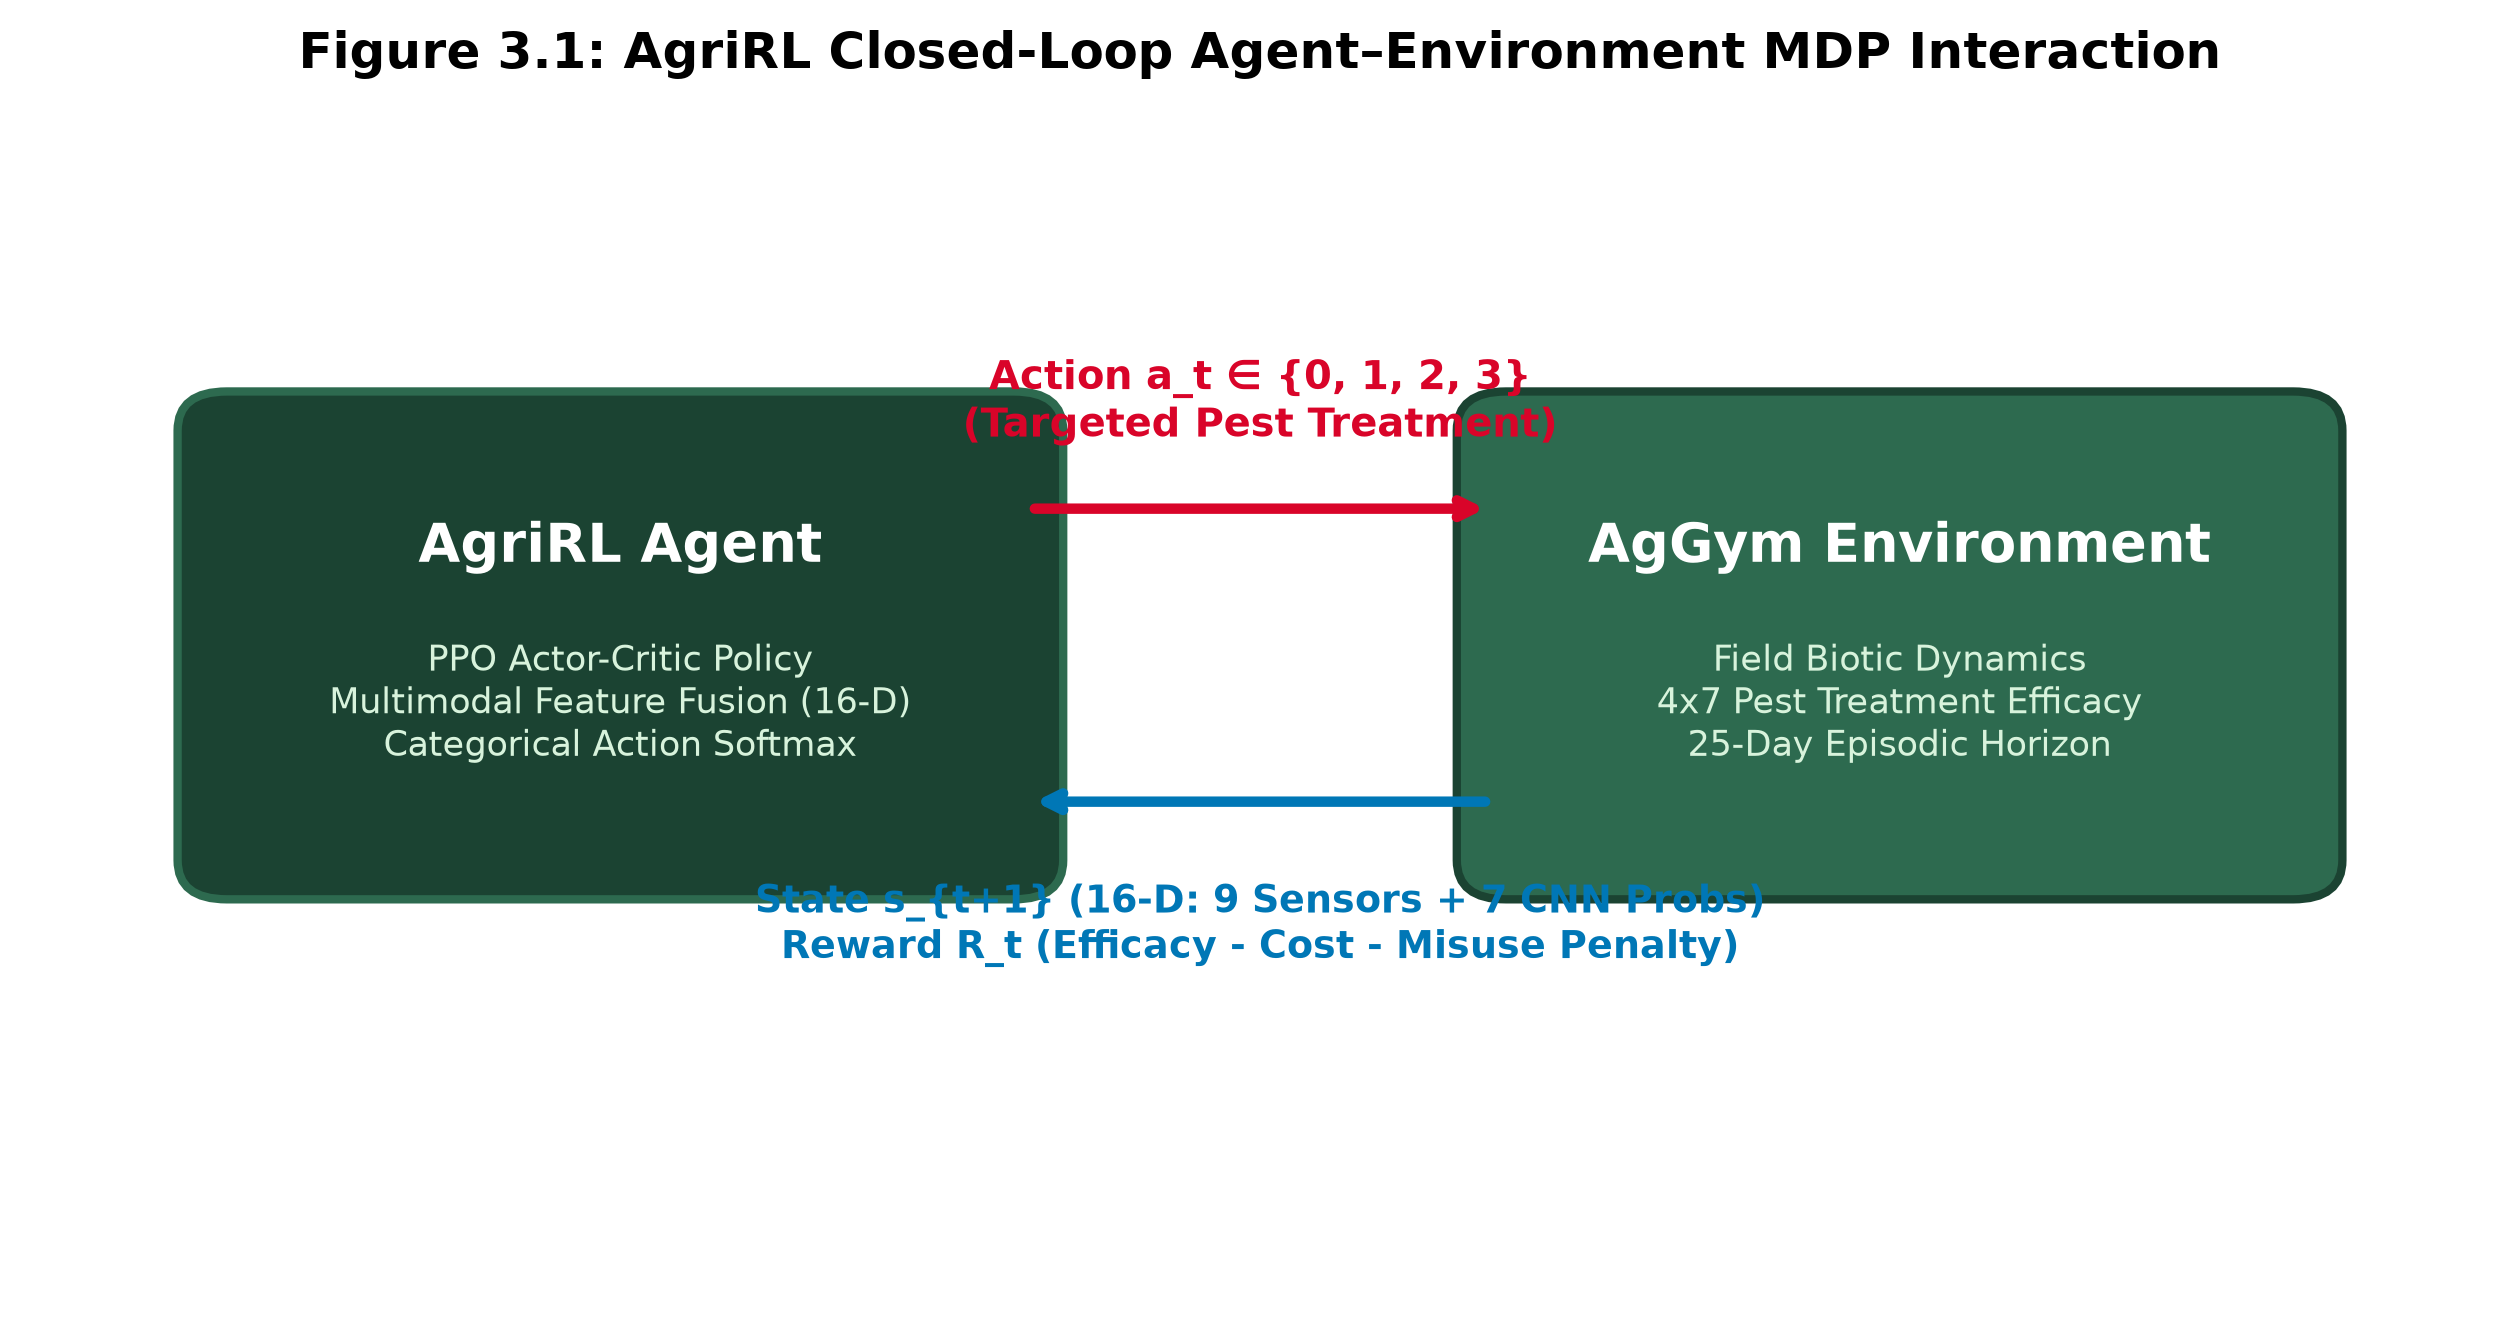
\includegraphics[width=0.85\textwidth]{img/fig_3_1_agent_environment.png}
\caption{AgriRL Closed-Loop Agent–Environment MDP Interaction Diagram}
\label{fig:agent_env}
\end{figure}

\section{Markov Decision Process Formulation}
Table~\ref{tab:mdp_formulation} defines the MDP components used in AgriRL.

\begin{table}[H]
\centering
\caption{Markov Decision Process Formulation Components}
\label{tab:mdp_formulation}
\begin{tabular}{p{3.5cm}p{11.5cm}}
\toprule
\textbf{MDP Component} & \textbf{Mathematical Definition in AgriRL} \\
\midrule
State Space $\mathcal{S}$ & 16-dimensional continuous vector: $s_t = [ x_t \text{ (9 sensor features)} \parallel p_t \text{ (7 CNN pest probabilities)} ] \in [0, 1]^{16}$ \\
Action Space $\mathcal{A}$ & Discrete set of 4 intervention actions: $\mathcal{A} = \{0: \text{None}, 1: \text{Low Bio}, 2: \text{Med Targeted}, 3: \text{High Broad-Spectrum}\}$ \\
Reward Function $R$ & $R(s, a, s') = 4.0 (\text{Pest}_t - \text{Pest}_{t+1}) + 2.5 \text{Health}_{t+1} - \text{Cost}(a) - \text{Penalty}_{\text{misuse}} + \text{Bonus}_{\text{harvest}}$ \\
Transition Dynamics $P$ & Stochastic transitions governing pest reproduction, natural mortality, and treatment knockdown \\
Discount Factor $\gamma$ & $\gamma = 0.95$ (balancing immediate chemical expense against long-term harvest payoff) \\
Episode Horizon $T$ & $T = 25$ daily discrete decision time-steps \\
\bottomrule
\end{tabular}
\end{table}

\section{State Space Representation}
The state space is a 16-dimensional continuous vector defined in $[0, 1]^{16}$:
\begin{itemize}
    \item \textbf{Dimensions 0 to 8 (Tabular Sensors):} $[\text{Pest\_Damage}/100, \text{Crop\_Health}/100, \text{Crop\_Stress}/100, \text{Temperature}/50, \text{Humidity}/100, \text{Soil\_Moisture}/100, \text{NDVI}, (\text{Growth\_Stage}-1)/3, \text{Hotspot\_Flag}]$.
    \item \textbf{Dimensions 9 to 15 (Vision CNN Probabilities):} $[p_{\text{aphid}}, p_{\text{armyworm}}, p_{\text{beetle}}, p_{\text{mite}}, p_{\text{sawfly}}, p_{\text{stem\_borer}}, p_{\text{stem\_fly}}]$ extracted via Softmax from the PyTorch CNN.
\end{itemize}

\section{Action Space Definition}
Table~\ref{tab:action_space} lists the four discrete actions with their costs and biological rationale.

\begin{table}[H]
\centering
\caption{Discrete Action Space Definitions, Chemical Costs, and Biological Rationale}
\label{tab:action_space}
\begin{tabular}{clll}
\toprule
\textbf{Action} & \textbf{Cost (\$)} & \textbf{Intervention Type} & \textbf{Targeted Biological Rationale} \\
\midrule
Action 0 & \$0.00 & No Treatment & Conserves expenditure when pest severity is $< 15\%$. \\
Action 1 & \$1.00 & Low Bio-Control & Neem oil / predator release; effective for Aphids and Mites. \\
Action 2 & \$2.00 & Med Targeted Chemical & Selective pesticide; targeted knockdown for defoliators. \\
Action 3 & \$3.00 & High Broad-Spectrum & High-dose emergency knockdown for deep borers / severe outbreaks. \\
\bottomrule
\end{tabular}
\end{table}

\section{Reward Function Design and Justification}
The multi-objective reward function incentivizes crop health preservation, penalizes operational expenditure, prevents chemical misuse, and rewards successful harvest completion:
\begin{equation}
R_t = 4.0 \max\left(0, \frac{\text{Pest}_t - \text{Pest}_{t+1}}{100}\right) + 2.5 \frac{\text{Health}_{t+1}}{100} - \text{Cost}(a_t) - \text{Penalty}_{\text{misuse}} + \text{Bonus}_{\text{harvest}}
\end{equation}
where $\text{Cost}(a) \in \{0, 1, 2, 3\}$, $\text{Penalty}_{\text{misuse}} = 2.0$ if Action 3 is applied when Pest $< 20\%$, and $\text{Bonus}_{\text{harvest}} = +50.0$ on Day 25 if $\text{Crop\_Health} \ge 70\%$.

\section{State Transition Dynamics}
Pest population dynamics follow an exponential reproduction curve attenuated by treatment efficacy:
\begin{equation}
\text{Pest}_{t+1} = \text{clip}\left(\text{Pest}_t (1.0 - \text{Efficacy}(a, p)) + \text{GrowthRate}(\text{Temp}, \text{Humidity}), 0.0, 100.0\right)
\end{equation}
where treatment efficacy is obtained from the $4 \times 7$ Pest-Treatment Efficacy Matrix $E[a, k]$ in Table~\ref{tab:efficacy_matrix}.

\begin{table}[H]
\centering
\caption{$4 \times 7$ Pest-Treatment Efficacy Matrix $E[a, k]$ in AgGym Simulation Environment}
\label{tab:efficacy_matrix}
\begin{tabular}{lccccccc}
\toprule
\textbf{Action} & \textbf{Aphid} & \textbf{Armyw.} & \textbf{Beetle} & \textbf{Mite} & \textbf{Sawfly} & \textbf{St.Bor.} & \textbf{St.Fly} \\
\midrule
0: None & 0.00 & 0.00 & 0.00 & 0.00 & 0.00 & 0.00 & 0.00 \\
1: Bio-Control & 0.80 & 0.20 & 0.25 & 0.75 & 0.25 & 0.15 & 0.20 \\
2: Targeted Chem & 0.65 & 0.85 & 0.80 & 0.60 & 0.85 & 0.85 & 0.80 \\
3: Broad-Spectrum & 0.90 & 0.95 & 0.92 & 0.88 & 0.92 & 0.95 & 0.92 \\
\bottomrule
\end{tabular}
\end{table}

\section{Initial and Terminal State Definition}
\textbf{Initial State:} Day 1, with initial pest severity drawn from preset agricultural scenarios (8\% to 88\%), crop health at 65--90\%, soil moisture at 25--55\%, and growth stage at Vegetative (Stage 1).

\textbf{Terminal State:} Day 25 reached (season harvest), or catastrophic crop failure ($\text{Crop\_Health} \le 0\%$).

\section{Episode Definition and Termination Conditions}
Each episode spans exactly 25 discrete daily decision steps corresponding to a complete agricultural crop cycle. Premature termination occurs if crop health collapses to 0.0\%.

\section{Assumptions and Constraints}
\begin{enumerate}
    \item Weather and microclimate telemetry follow calibrated distributions drawn from the Kaggle Agricultural Dataset.
    \item The 7 pest species represent the dominant biotic threats in crop cultivation.
    \item The agent operates as a software advisory recommendation engine and does not execute physical spray actuation.
\end{enumerate}

% -------------------------------------------------------------
% CHAPTER 4: PROPOSED REINFORCEMENT LEARNING METHODOLOGY
% -------------------------------------------------------------
\chapter{Proposed Reinforcement Learning Methodology}

\section{Overview of the Proposed Methodology}
AgriRL applies an on-policy Actor-Critic Proximal Policy Optimization (PPO) architecture operating over a continuous 16-dimensional observation vector constructed via Late Vector Fusion of vision and telemetry features.

\section{Selection and Justification of RL Algorithm}
Table~\ref{tab:rl_comparison} details the algorithm comparison and rationale.

\begin{table}[H]
\centering
\caption{Algorithm Comparison, Rationale, Advantages, and Trade-offs}
\label{tab:rl_comparison}
\begin{tabular}{p{3.0cm}p{3.2cm}p{4.2cm}p{4.2cm}}
\toprule
\textbf{Algorithm} & \textbf{Why Selected / Tested} & \textbf{Advantages} & \textbf{Limitations} \\
\midrule
Random Baseline & Zero-intelligence benchmark & Provides statistical performance floor & Severe over-spraying; low returns \\
Tabular-Only PPO & Baseline (sensors only) & Optimizes climate variables well & Species-blind; sprays wrong chemicals \\
Multimodal PPO (Proposed) & Final multimodal model & Pest-aware; optimal chemical conservation & Requires lightweight CNN inference \\
\bottomrule
\end{tabular}
\end{table}

\section{Mathematical Foundation of the Algorithm}
PPO optimizes a clipped surrogate objective function that prevents destructively large policy updates [1]:
\begin{equation}
L^{\text{CLIP}}(\theta) = \hat{\mathbb{E}}_t \left[ \min\left( r_t(\theta)\hat{A}_t, \, \text{clip}(r_t(\theta), 1-\epsilon, 1+\epsilon)\hat{A}_t \right) \right]
\end{equation}
where $r_t(\theta) = \frac{\pi_\theta(a_t | s_t)}{\pi_{\theta_{\text{old}}}(a_t | s_t)}$, $\epsilon = 0.2$ is the clipping parameter, and $\hat{A}_t$ is Generalized Advantage Estimation (GAE) [11]:
\begin{equation}
\hat{A}_t^{\text{GAE}} = \sum_{l=0}^\infty (\gamma \lambda)^l \delta_{t+l}^V
\end{equation}

\begin{figure}[H]
\centering
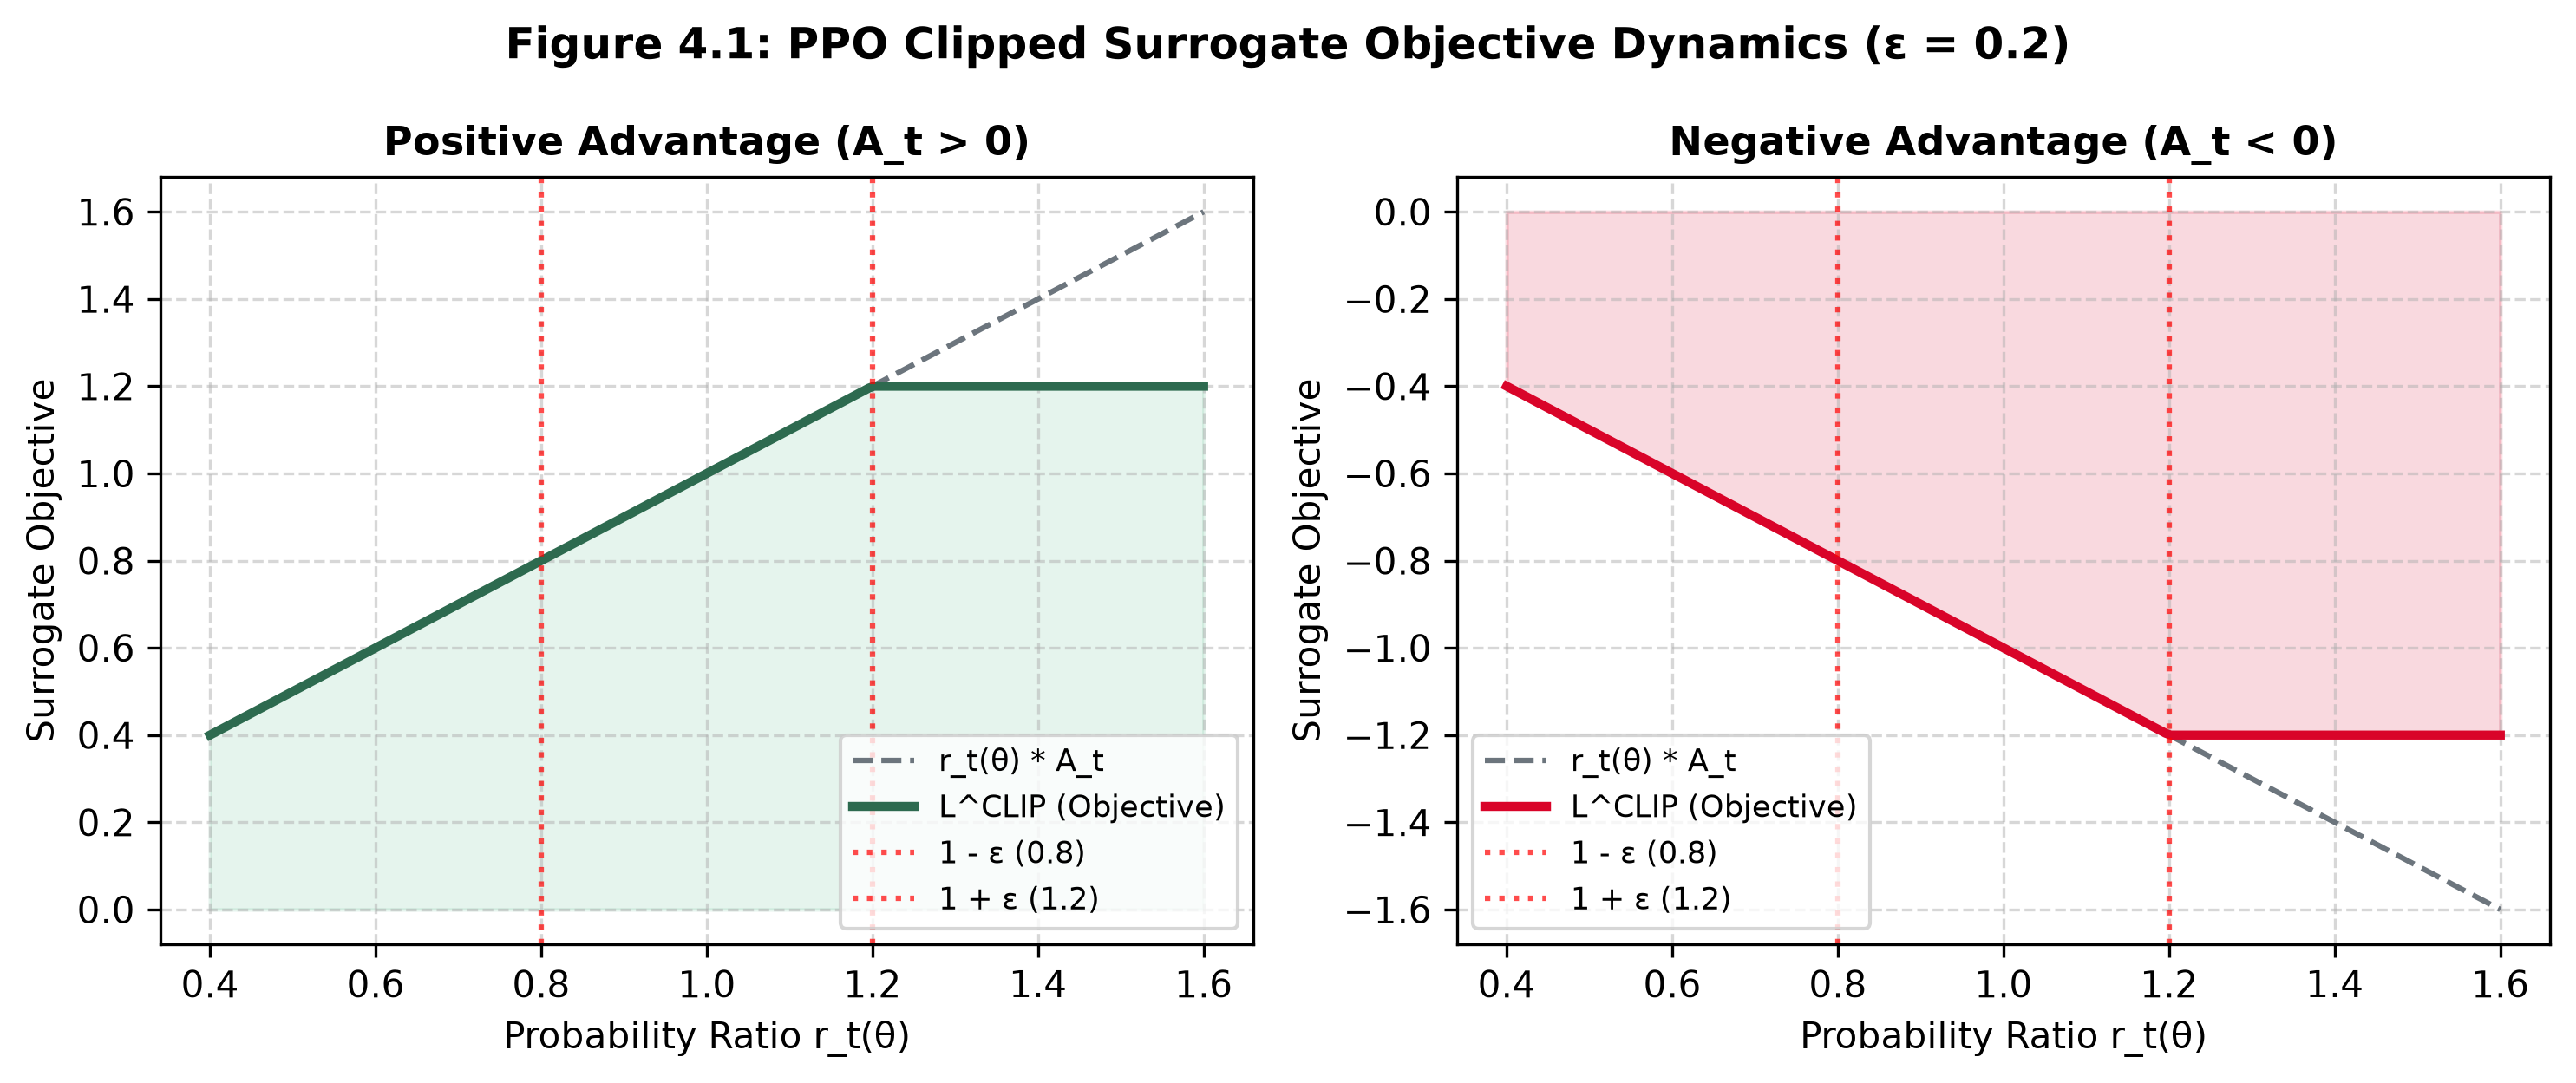
\includegraphics[width=0.85\textwidth]{img/fig_4_2_ppo_clipped_objective.png}
\caption{PPO Clipped Surrogate Objective and Policy Update Mechanism ($\epsilon = 0.2$)}
\label{fig:ppo_clipped}
\end{figure}

\section{Agent Architecture}
The PPO agent employs separate Actor and Critic Multi-Layer Perceptrons (MLPs), shown in Figure~\ref{fig:multimodal_arch}:
\begin{itemize}
    \item \textbf{Shared Input Layer:} 16 continuous neurons.
    \item \textbf{Hidden Layer 1:} 64 neurons with Tanh activation.
    \item \textbf{Hidden Layer 2:} 64 neurons with Tanh activation.
    \item \textbf{Actor Output:} 4 discrete action logits passed through Softmax.
    \item \textbf{Critic Output:} 1 scalar state-value estimate $V(s)$.
\end{itemize}

\begin{figure}[H]
\centering
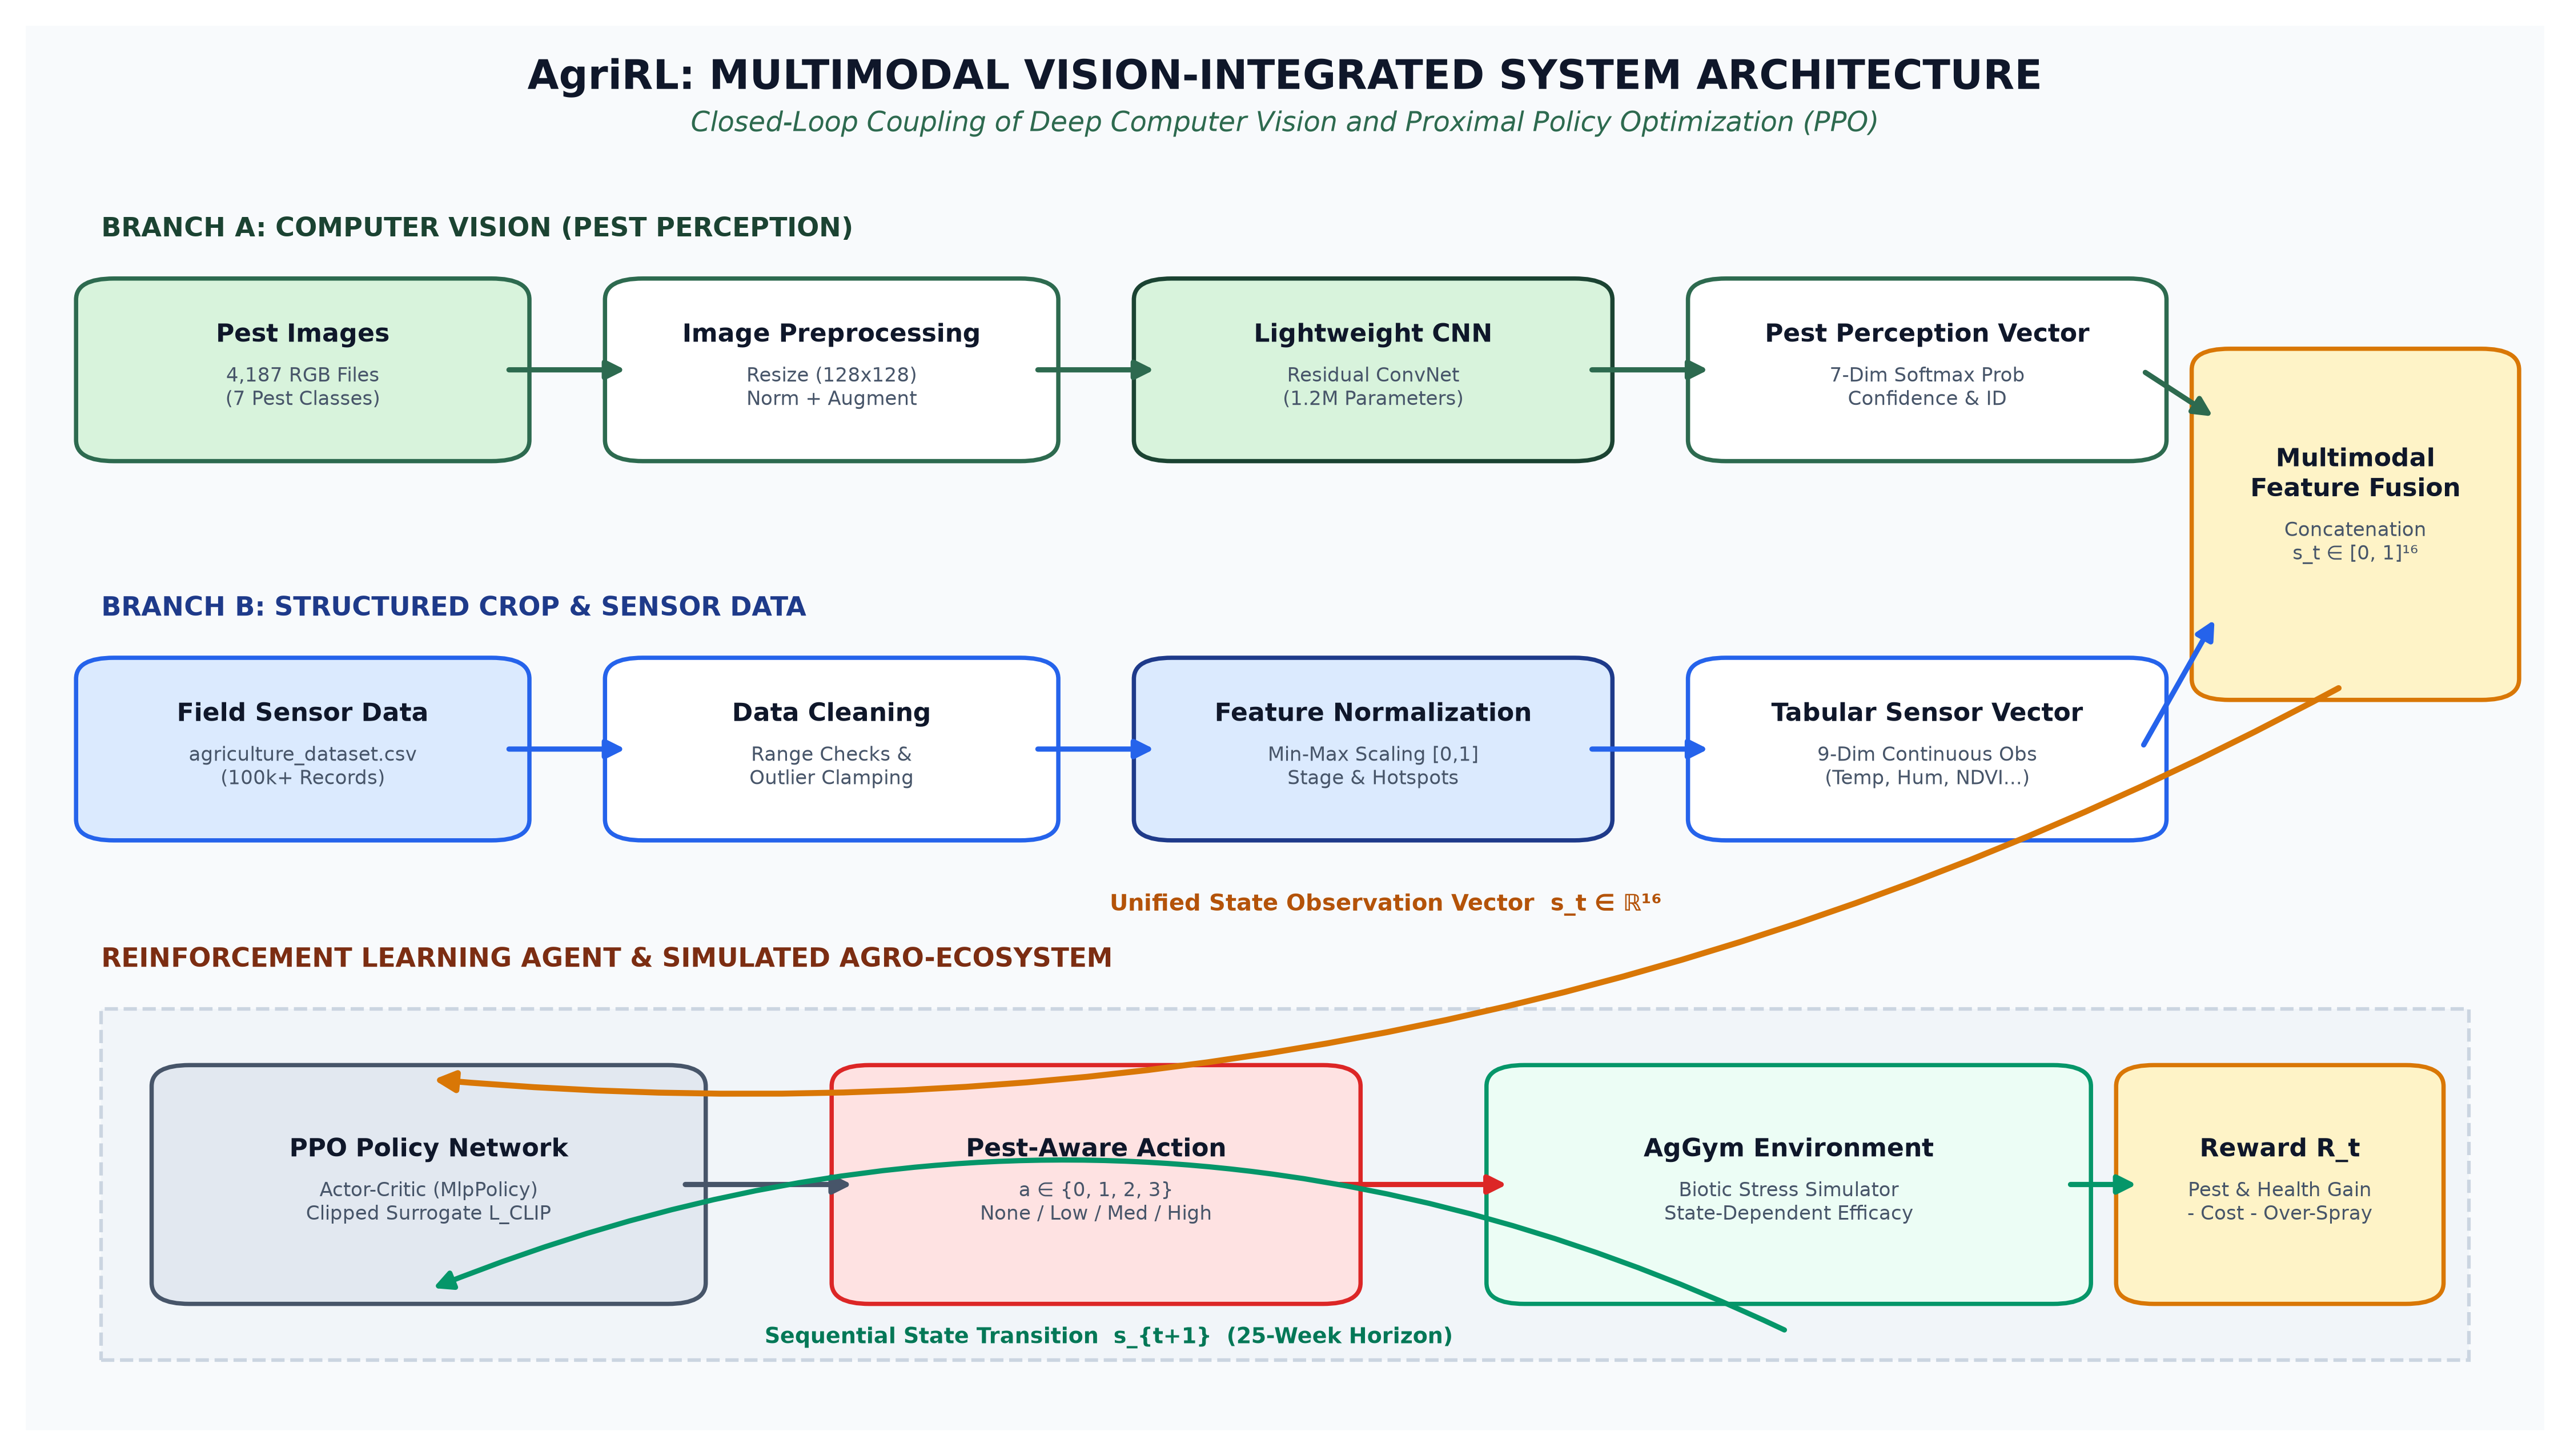
\includegraphics[width=0.85\textwidth]{img/fig_4_1_multimodal_architecture.png}
\caption{Multimodal Dual-Branch Actor-Critic Neural Architecture}
\label{fig:multimodal_arch}
\end{figure}

\section{Policy Representation}
The policy $\pi_\theta(a | s)$ is parameterized as a categorical probability distribution over the 4 actions. Action selection during evaluation is deterministic ($\text{argmax}$), while during training it is sampled stochastically.

\section{Value Function / Q-Function Estimation}
The Critic network estimates the expected discounted return:
\begin{equation}
V(s_t) = \mathbb{E}\left[ \sum_{k=0}^\infty \gamma^k R_{t+k+1} \,\middle|\, s_t \right]
\end{equation}
updated via Mean Squared Error (MSE) against empirical return targets.

\section{Exploration–Exploitation Strategy}
Exploration is driven by an explicit Policy Entropy Bonus added to the objective:
\begin{equation}
L_{\text{total}} = L^{\text{CLIP}} - c_1 L^{\text{VF}} + c_2 \mathcal{H}(\pi_\theta)
\end{equation}
The entropy coefficient $c_2 = 0.01$ encourages active exploration during initial steps and smoothly decays as the policy converges.

\section{Learning and Policy Update Mechanism}
Trajectories are gathered across 2,048 steps per rollout. The collected transitions are segmented into mini-batches of size 64 and optimized across 10 epochs using the Adam optimizer with gradient clipping at 0.5.

\section{Hyperparameter Selection}
Table~\ref{tab:hyperparams} summarizes the configured PPO hyperparameters.

\begin{table}[H]
\centering
\caption{PPO Hyperparameter Specifications and Training Constants}
\label{tab:hyperparams}
\begin{tabular}{lll}
\toprule
\textbf{Hyperparameter} & \textbf{Configured Value} & \textbf{Operational Meaning} \\
\midrule
Discount Factor ($\gamma$) & 0.95 & Discounting of future ecological returns \\
GAE Parameter ($\lambda$) & 0.95 & Variance-bias trade-off for advantage \\
PPO Clip Range ($\epsilon$) & 0.20 & Clipping threshold for probability ratio \\
Learning Rate ($\alpha$) & $3 \times 10^{-4}$ & Adam optimizer step size \\
Entropy Coefficient & 0.01 & Weight of policy entropy exploration bonus \\
Rollout Buffer Size & 2,048 steps & Experience gathered per policy update \\
Mini-Batch Size & 64 & Stochastic gradient descent batch size \\
Optimization Epochs & 10 & SGD passes per rollout buffer \\
Total Training Budget & 15,000 steps & Matched budget across all multi-seed runs \\
\bottomrule
\end{tabular}
\end{table}

\section{Algorithmic Workflow and Pseudocode}
\begin{tabbing}
\textbf{Algorithm 1:} Multimodal Vision-Integrated PPO Training \\
1: \quad Initialize PPO Actor-Critic weights $\theta, \phi$ and CNN weights $\psi$ \\
2: \quad \textbf{for} iteration = 1 to $N$ \textbf{do} \\
3: \quad\quad \textbf{for} step = 1 to 2048 \textbf{do} \\
4: \quad\quad\quad Observe image $I_t$ and sensor vector $x_t$ \\
5: \quad\quad\quad Compute $p_t = \text{Softmax}(\text{CNN}_\psi(I_t))$ \\
6: \quad\quad\quad Form multimodal state $s_t = [x_t \parallel p_t]$ \\
7: \quad\quad\quad Sample action $a_t \sim \pi_\theta(a | s_t)$, evaluate value $V_\phi(s_t)$ \\
8: \quad\quad\quad Execute $a_t$ in AgGymWrapperEnv; receive $r_t, s_{t+1}, \text{done}$ \\
9: \quad\quad\quad Store transition $(s_t, a_t, r_t, V_\phi, \log \pi)$ in buffer \\
10: \quad\quad \textbf{end for} \\
11: \quad\quad Compute GAE advantages $\hat{A}_t^{\text{GAE}}$ and returns \\
12: \quad\quad \textbf{for} epoch = 1 to 10 \textbf{do} \\
13: \quad\quad\quad Update $\theta$ via clipped surrogate objective $L^{\text{CLIP}}$ \\
14: \quad\quad\quad Update $\phi$ via MSE value loss $L^{\text{VF}}$ \\
15: \quad\quad \textbf{end for} \\
16: \quad \textbf{end for}
\end{tabbing}

\section{Computational Complexity Analysis}
Per-step inference complexity is $\mathcal{O}(1)$ for the PPO MLP forward pass (5,639 parameters). CNN feature extraction on $128 \times 128$ images requires 1.2M floating-point operations ($\sim 12$ ms on CPU). The total 15,000-step training executes in $\sim 38$ seconds on standard CPU hardware.

% -------------------------------------------------------------
% CHAPTER 5: SYSTEM DESIGN AND IMPLEMENTATION
% -------------------------------------------------------------
\chapter{System Design and Implementation}

\section{Overall System Architecture}
The system architecture comprises three modular layers: (1) Computer Vision Preprocessing \& Classification Layer, (2) Gymnasium Environment Simulation Layer (\texttt{AgGymWrapperEnv}), and (3) PPO Policy Controller \& Web Presentation Layer (Figure~\ref{fig:sys_arch}).

\begin{figure}[H]
\centering
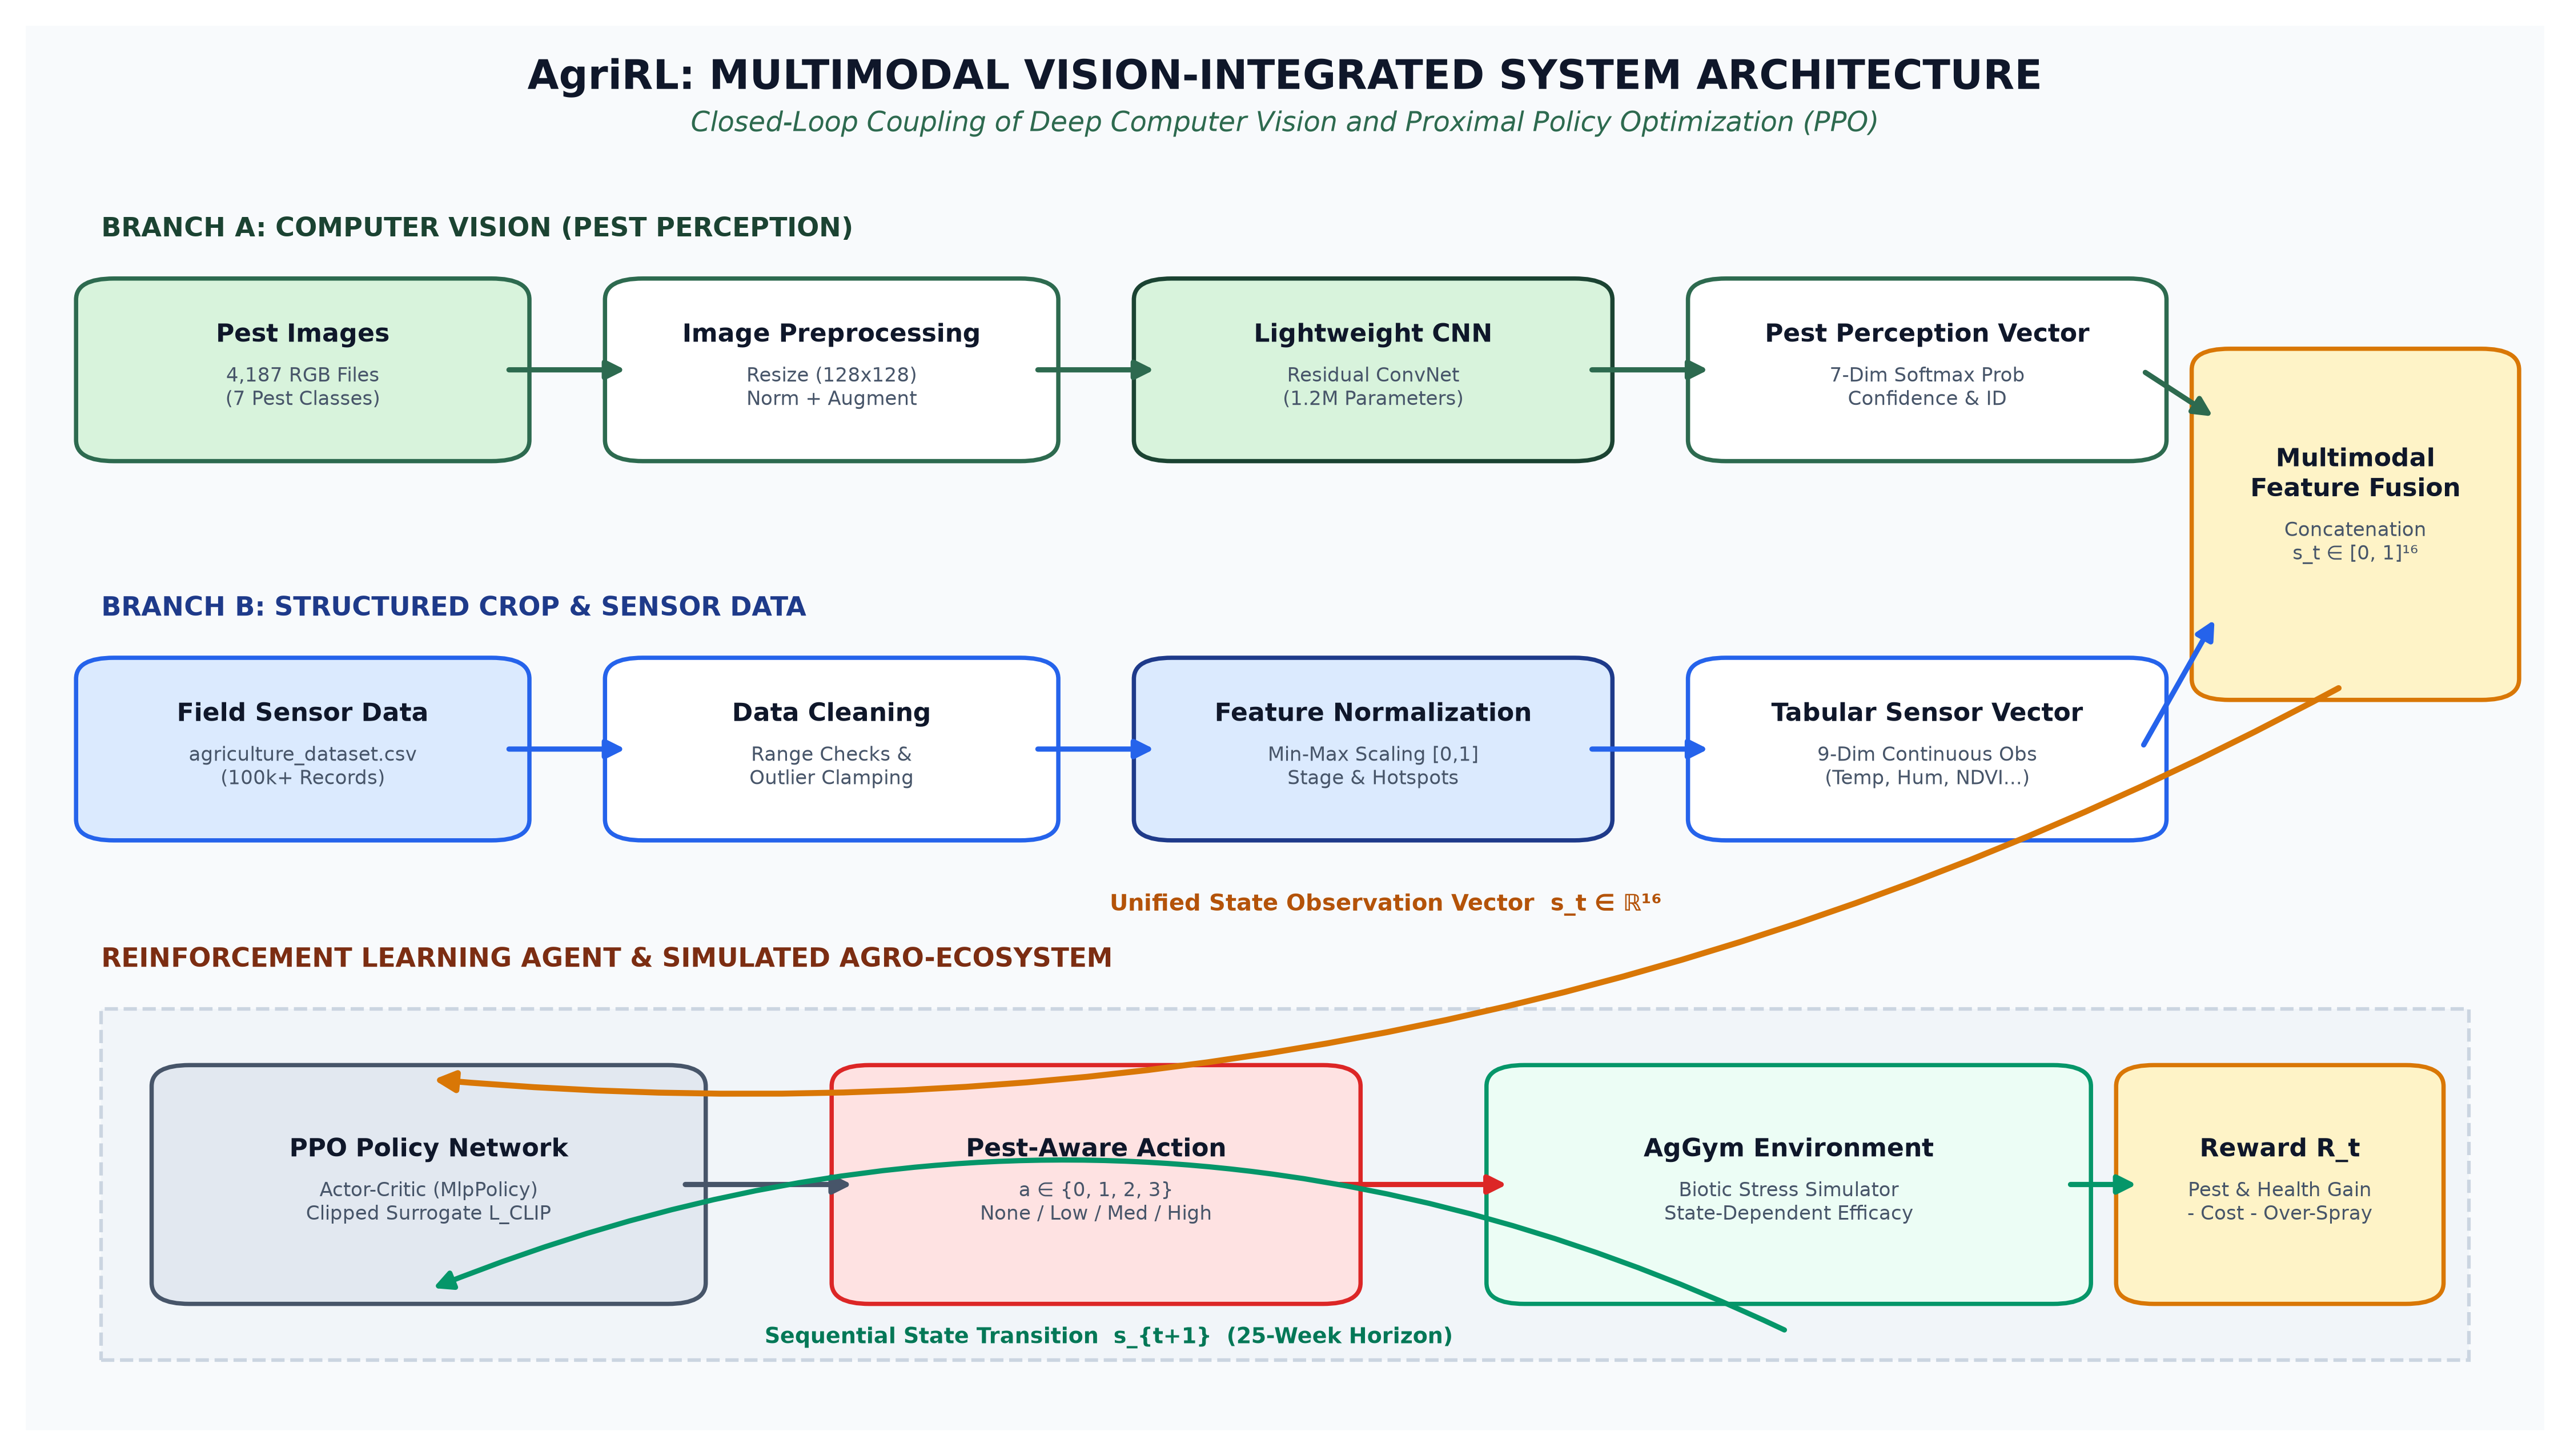
\includegraphics[width=0.85\textwidth]{img/fig_5_1_system_architecture.png}
\caption{Overall AgriRL System Architecture Diagram}
\label{fig:sys_arch}
\end{figure}

\section{Software and Hardware Requirements}
\section{Development Environment and Libraries}
Development followed modern Gymnasium [16] and Stable-Baselines3 [15] conventions. Due to torchvision version incompatibilities in Python 3.14, the vision pipeline was custom-engineered using pure PyTorch neural blocks and Pillow transforms, ensuring complete dependency isolation (Table~\ref{tab:reqs}).

\begin{table}[H]
\centering
\caption{Software, Hardware, and Library Requirements}
\label{tab:reqs}
\begin{tabular}{ll}
\toprule
\textbf{Item} & \textbf{Specification} \\
\midrule
Operating System & Microsoft Windows 11 / Linux Ubuntu 22.04 LTS \\
Programming Language & Python 3.10 / 3.12 / 3.14 \\
Core ML Libraries & PyTorch, Gymnasium, Stable-Baselines3, NumPy, Pandas, Scikit-Learn \\
Computer Vision & Pillow (PIL), NumPy (torchvision-free standalone implementation) \\
Web Framework & Python Multi-Threaded HTTPServer (\texttt{ThreadedHTTPServer}), HTML5, CSS3, JS \\
Hardware Minimum & Intel Core i5 / AMD Ryzen 5, 8 GB RAM, standard CPU (no GPU required) \\
\bottomrule
\end{tabular}
\end{table}

\section{Environment Design and Configuration}
\texttt{AgGymWrapperEnv} wraps agricultural stress dynamics with realistic environmental degradation, pesticide efficacy attenuation, natural mortality, and economic penalty calculations. Pre-computed class probability distributions are cached in \texttt{models/pest\_prob\_cache.npz}.

\section{State and Action Encoding}
Observations are mapped into a $\text{Box}(16,)$ continuous space. Actions are discrete integers $\{0, 1, 2, 3\}$. All state variables are normalized to $[0, 1]$. Table~\ref{tab:state_enc} gives the feature encoding of the 16-dimensional state vector.

\begin{table}[H]
\centering
\caption{16-Dimensional Multimodal State Vector Feature Encoding}
\label{tab:state_enc}
\begin{tabular}{lll}
\toprule
\textbf{Index} & \textbf{Source} & \textbf{Feature (Normalization)} \\
\midrule
0 & Sensor & $\text{Pest\_Damage} / 100$ \\
1 & Sensor & $\text{Crop\_Health} / 100$ \\
2 & Sensor & $\text{Crop\_Stress} / 100$ \\
3 & Sensor & $\text{Temperature} / 50$ \\
4 & Sensor & $\text{Humidity} / 100$ \\
5 & Sensor & $\text{Soil\_Moisture} / 100$ \\
6 & Sensor & $\text{NDVI}$ \\
7 & Sensor & $(\text{Growth\_Stage} - 1) / 3$ \\
8 & Sensor & $\text{Hotspot\_Flag}$ \\
9--15 & Vision CNN & Softmax probabilities: aphid, armyworm, beetle, mite, sawfly, stem borer, stem fly \\
\bottomrule
\end{tabular}
\end{table}

\section{Reward Function Implementation}
The multi-objective reward is implemented in \texttt{env\_aggym\_wrapper.py}, directly penalizing operational costs, rewarding pest reduction, and assigning terminal harvest bonuses.

\section{Agent Implementation}
The agent is implemented via Stable-Baselines3 PPO with a custom \texttt{MlpPolicy} architecture. Action selection supports both deterministic evaluation and stochastic sampling with temperature scaling.

\section{Training Pipeline}
The master training engine (\texttt{train\_and\_eval.py}) executes matched-budget multi-seed protocols across Seeds 0, 1, and 2, recording comprehensive training histories, moving averages, and diagnostic metrics.

\section{Model Saving and Loading}
Trained models are saved to disk as \texttt{models/pest\_cnn.pt} (PyTorch state dict) and \texttt{models/multimodal\_vision\_ppo.zip} (Stable-Baselines3 archive), enabling fast loading in the web simulator in $< 200$ ms.

\section{Testing and Validation}
Validation was conducted via: (1) stratified test-set image classification on 630 held-out images, (2) 30 evaluation episodes per seed on unseen field plots, (3) Robustness Gap stress testing under noise perturbations, and (4) live web simulator execution. Figures~\ref{fig:web_dash}--\ref{fig:web_eco} show the interactive web application.

\begin{figure}[H]
\centering
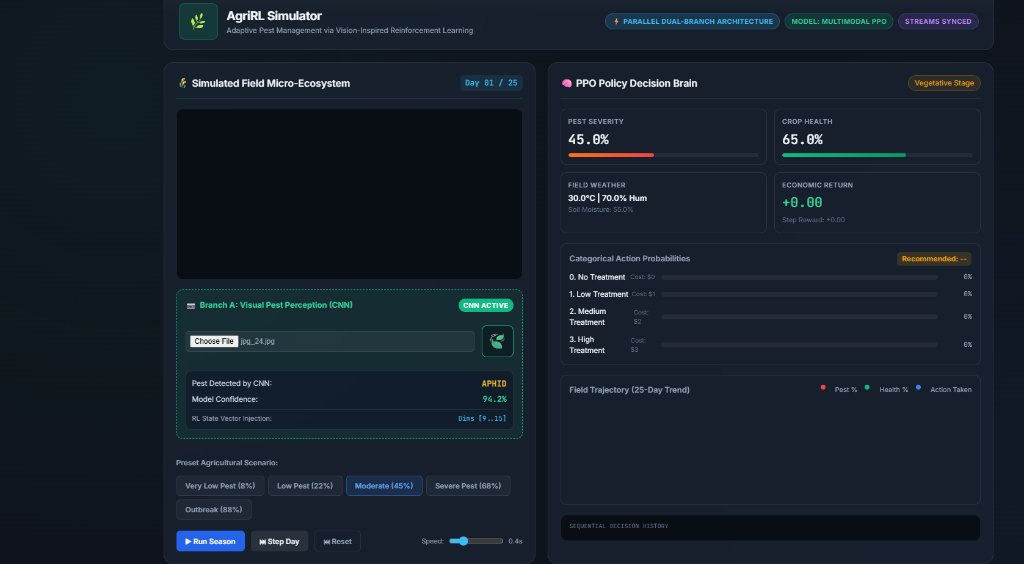
\includegraphics[width=0.85\textwidth]{img/fig_5_2_web_dashboard.png}
\caption{Web Application Dashboard: Dual-Stream Observation and Telemetry}
\label{fig:web_dash}
\end{figure}

\begin{figure}[H]
\centering
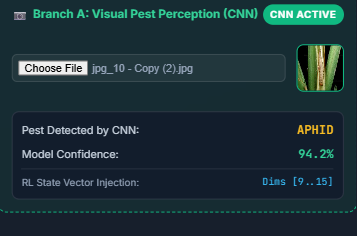
\includegraphics[width=0.75\textwidth]{img/fig_5_3_web_leaf_upload.png}
\caption{Web Application: Leaf Upload, Live CNN Classification and PPO Action Rationale}
\label{fig:web_leaf}
\end{figure}

\begin{figure}[H]
\centering
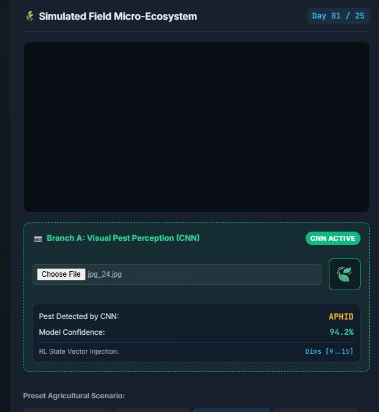
\includegraphics[width=0.75\textwidth]{img/fig_5_4_web_ecosystem.png}
\caption{Web Application: 48-Tile Micro-Ecosystem and Chemical Spray Animation}
\label{fig:web_eco}
\end{figure}

% -------------------------------------------------------------
% CHAPTER 6: EXPERIMENTAL SETUP AND EVALUATION
% -------------------------------------------------------------
\chapter{Experimental Setup and Evaluation}

\section{Experimental Objectives}
\begin{enumerate}
    \item Quantify the performance improvement of Multimodal Vision PPO over Tabular PPO and Random baselines.
    \item Evaluate CNN classification accuracy, Macro-F1, and confusion matrix on the 7-class pest dataset.
    \item Measure chemical over-spray reduction and harvest success rate across random seeds.
    \item Analyze policy exploration schedules via Shannon entropy decay.
\end{enumerate}

\section{Dataset / Environment Description}
The vision branch uses the Kaggle Pest Detection dataset [19] (4,187 images, 7 classes) and the tabular branch uses the Agricultural Crop Health dataset [20]. Table~\ref{tab:pest_dataset} lists the class distribution and the stratified 70:15:15 split.

\begin{table}[H]
\centering
\caption{Kaggle Pest Detection Dataset Class Distribution and Stratified 70:15:15 Split}
\label{tab:pest_dataset}
\begin{tabular}{lcccc}
\toprule
\textbf{Pest Species} & \textbf{Total Images} & \textbf{Train (70\%)} & \textbf{Val (15\%)} & \textbf{Test (15\%)} \\
\midrule
Aphid & 1,303 & 912 & 195 & 196 \\
Armyworm & 350 & 245 & 52 & 53 \\
Beetle & 350 & 245 & 52 & 53 \\
Mite & 1,200 & 840 & 180 & 180 \\
Sawfly & 350 & 245 & 52 & 53 \\
Stem Borer & 350 & 245 & 52 & 53 \\
Stem Fly & 284 & 199 & 43 & 42 \\
\midrule
\textbf{Total} & \textbf{4,187} & \textbf{2,931} & \textbf{626} & \textbf{630} \\
\bottomrule
\end{tabular}
\end{table}

\section{Experimental Configuration}
\section{Training Parameters and Hyperparameters}
All algorithms were trained under identical computational budgets: 15,000 environment steps per run across 3 independent random seeds (Seeds 0, 1, 2) on the same CPU hardware. Table~\ref{tab:eval_protocol} outlines the protocol.

\begin{table}[H]
\centering
\caption{Experimental Parameters and Multi-Seed Evaluation Protocol}
\label{tab:eval_protocol}
\begin{tabular}{ll}
\toprule
\textbf{Component} & \textbf{Configuration} \\
\midrule
CNN Training & 50 epochs, batch size 64, Adam optimizer, $\text{lr} = 0.001$ with CosineAnnealingLR \\
PPO Training & $\gamma = 0.95$, $\text{lr} = 0.0003$, $\text{clip} = 0.2$, GAE $\lambda = 0.95$, entropy coeff $= 0.01$ \\
Training Budget & 15,000 environment steps per run (matched across methods) \\
Independent Seeds & 3 (Seeds 0, 1, 2) \\
Evaluation Episodes & 30 deterministic test episodes per seed (90 per model family) \\
\bottomrule
\end{tabular}
\end{table}

\section{Number of Training Episodes and Independent Runs}
Each model was trained across 3 independent seeds. Each seed was evaluated over 30 deterministic test episodes on unseen environmental seeds (total 90 test episodes per model family).

\section{Evaluation Metrics}
Table~\ref{tab:eval_metrics} defines the evaluation metrics.

\begin{table}[H]
\centering
\caption{Evaluation Metrics, Definitions, and Justifications}
\label{tab:eval_metrics}
\begin{tabular}{lll}
\toprule
\textbf{Metric} & \textbf{Definition} & \textbf{Target Goal} \\
\midrule
Cumulative Return & Sum of undiscounted rewards per 25-day season & Maximize ($> 65.0$) \\
Harvest Success Rate (\%) & Share of episodes ending with Health $\ge 70\%$ & Maximize ($> 50\%$) \\
Violation Rate (\%) & Share of steps with unnecessary Action 3 spraying & Minimize ($< 30\%$) \\
Robustness Gap & Difference in return between nominal and noisy inputs & Minimize ($< 2.0$) \\
Policy Entropy (nats) & Shannon entropy of action probability distribution & Smooth decay \\
\bottomrule
\end{tabular}
\end{table}

\section{Baseline Methods for Comparison}
\begin{enumerate}
    \item \textbf{Random Policy:} Selects actions uniformly at random; represents the absence of control.
    \item \textbf{Tabular-Only PPO:} Mini-project baseline that observes only the 9 environmental features without pest species identity.
\end{enumerate}

\section{Experimental Scenarios and Test Cases}
Policies were evaluated across 5 agricultural infestation levels: Very Low (8\% pest), Low (22\% pest), Moderate (45\% pest), Severe (68\% pest), and Outbreak (88\% pest).

\section{Evaluation Protocol}
Evaluation was conducted strictly on held-out test splits with deterministic policy execution (\texttt{deterministic=True}) and reported with 95\% Confidence Intervals: $\text{Mean} \pm 1.96 (\sigma / \sqrt{N})$.

% -------------------------------------------------------------
% CHAPTER 7: RESULTS AND DISCUSSION
% -------------------------------------------------------------
\chapter{Results and Discussion}

\section{Training Performance Analysis}
Training logs reveal rapid convergence for Multimodal PPO, surpassing the Tabular baseline within 4,000 steps and reaching a stable plateau of $\sim 69.0$ return.

\section{Cumulative Reward Analysis}
Table~\ref{tab:headline_results} presents the headline multi-seed results.

\begin{table}[H]
\centering
\caption{Headline Multi-Seed Experimental Results: Random vs. Tabular PPO vs. Multimodal PPO}
\label{tab:headline_results}
\begin{tabular}{lccc}
\toprule
\textbf{Model / Policy} & \textbf{Return (Mean $\pm$ Std)} & \textbf{Success Rate (\%)} & \textbf{Violation Rate (\%)} \\
\midrule
Random Baseline & $20.24 \pm 2.20$ & 34.4 & 58.7 \\
Tabular-Only PPO (Mini-Project) & $60.29 \pm 11.56$ & 2.2 & 0.0 \\
\textbf{Multimodal Vision PPO (Final)} & $\mathbf{68.69 \pm 2.11}$ & \textbf{56.7} & \textbf{27.0} \\
\bottomrule
\end{tabular}
\end{table}

\begin{figure}[H]
\centering
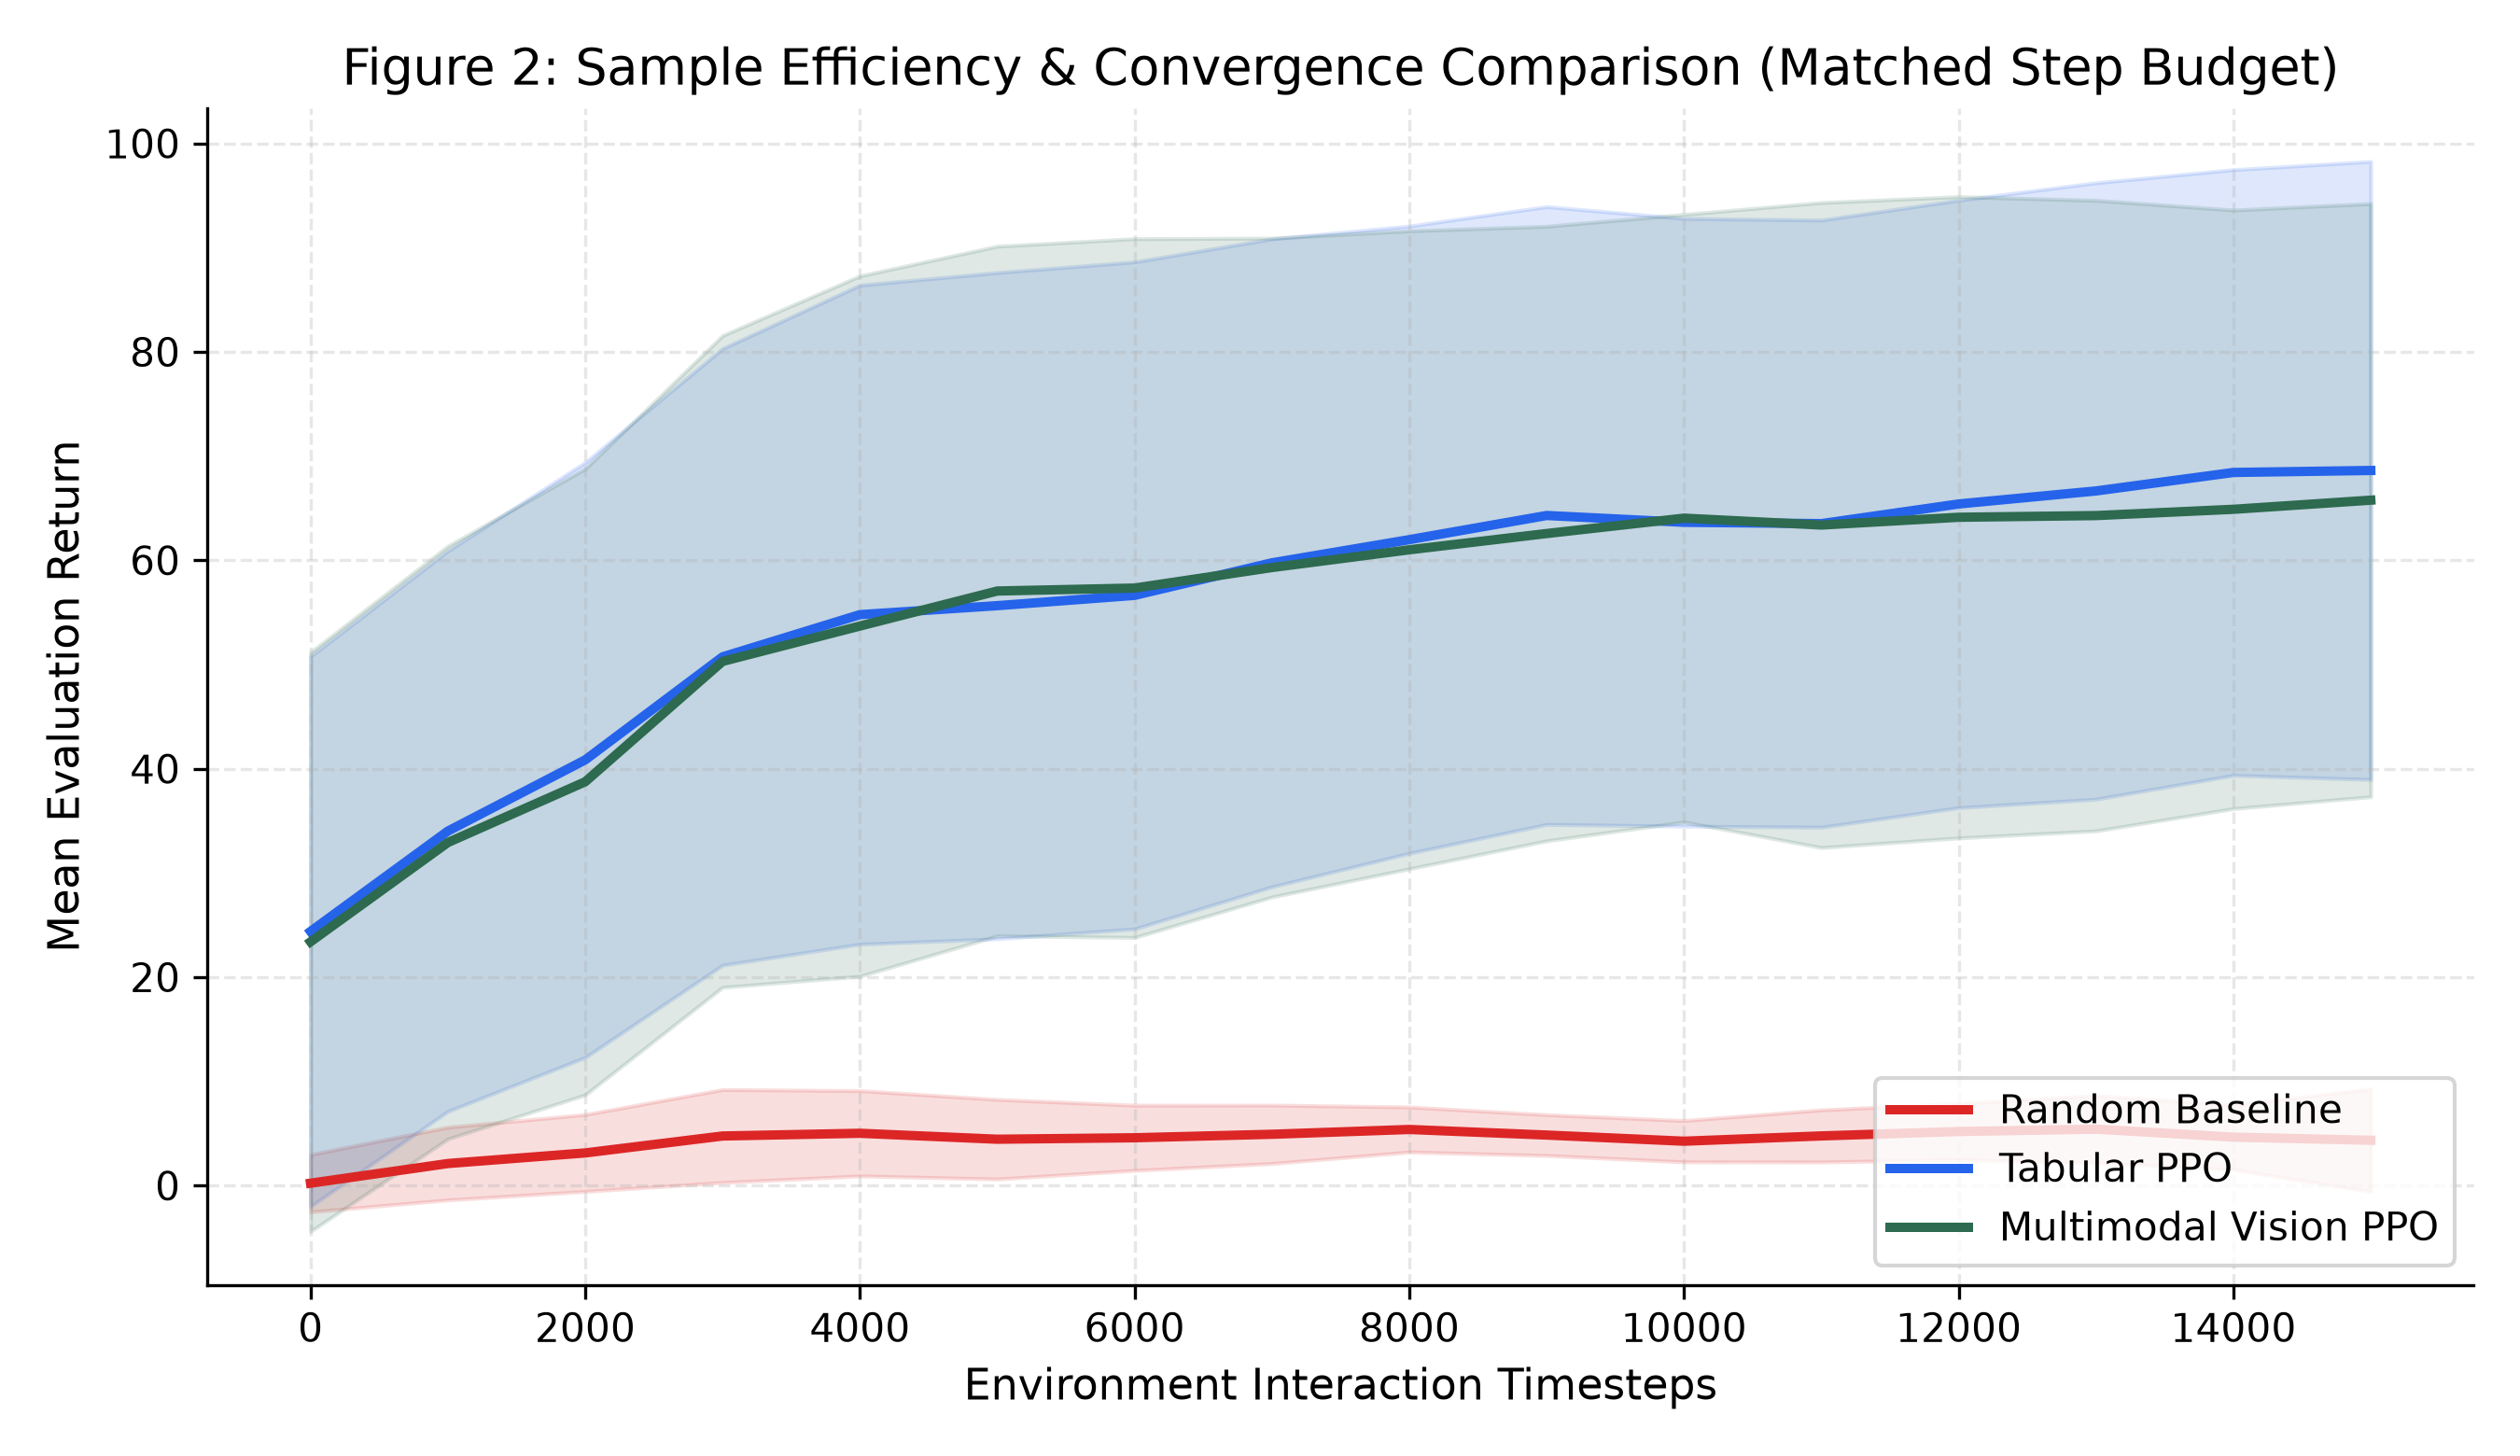
\includegraphics[width=0.85\textwidth]{img/fig_7_1_baseline_comparison.png}
\caption{Baseline Comparison Across Matched Budget: Random vs. Tabular vs. Multimodal PPO}
\label{fig:baseline_comp}
\end{figure}

\section{Learning Curve and Convergence Behaviour}
Figure~\ref{fig:learning_curves} illustrates episode returns and 50-episode moving averages across training. Multimodal PPO exhibits smooth monotonic improvement without catastrophic forgetting.

\begin{figure}[H]
\centering
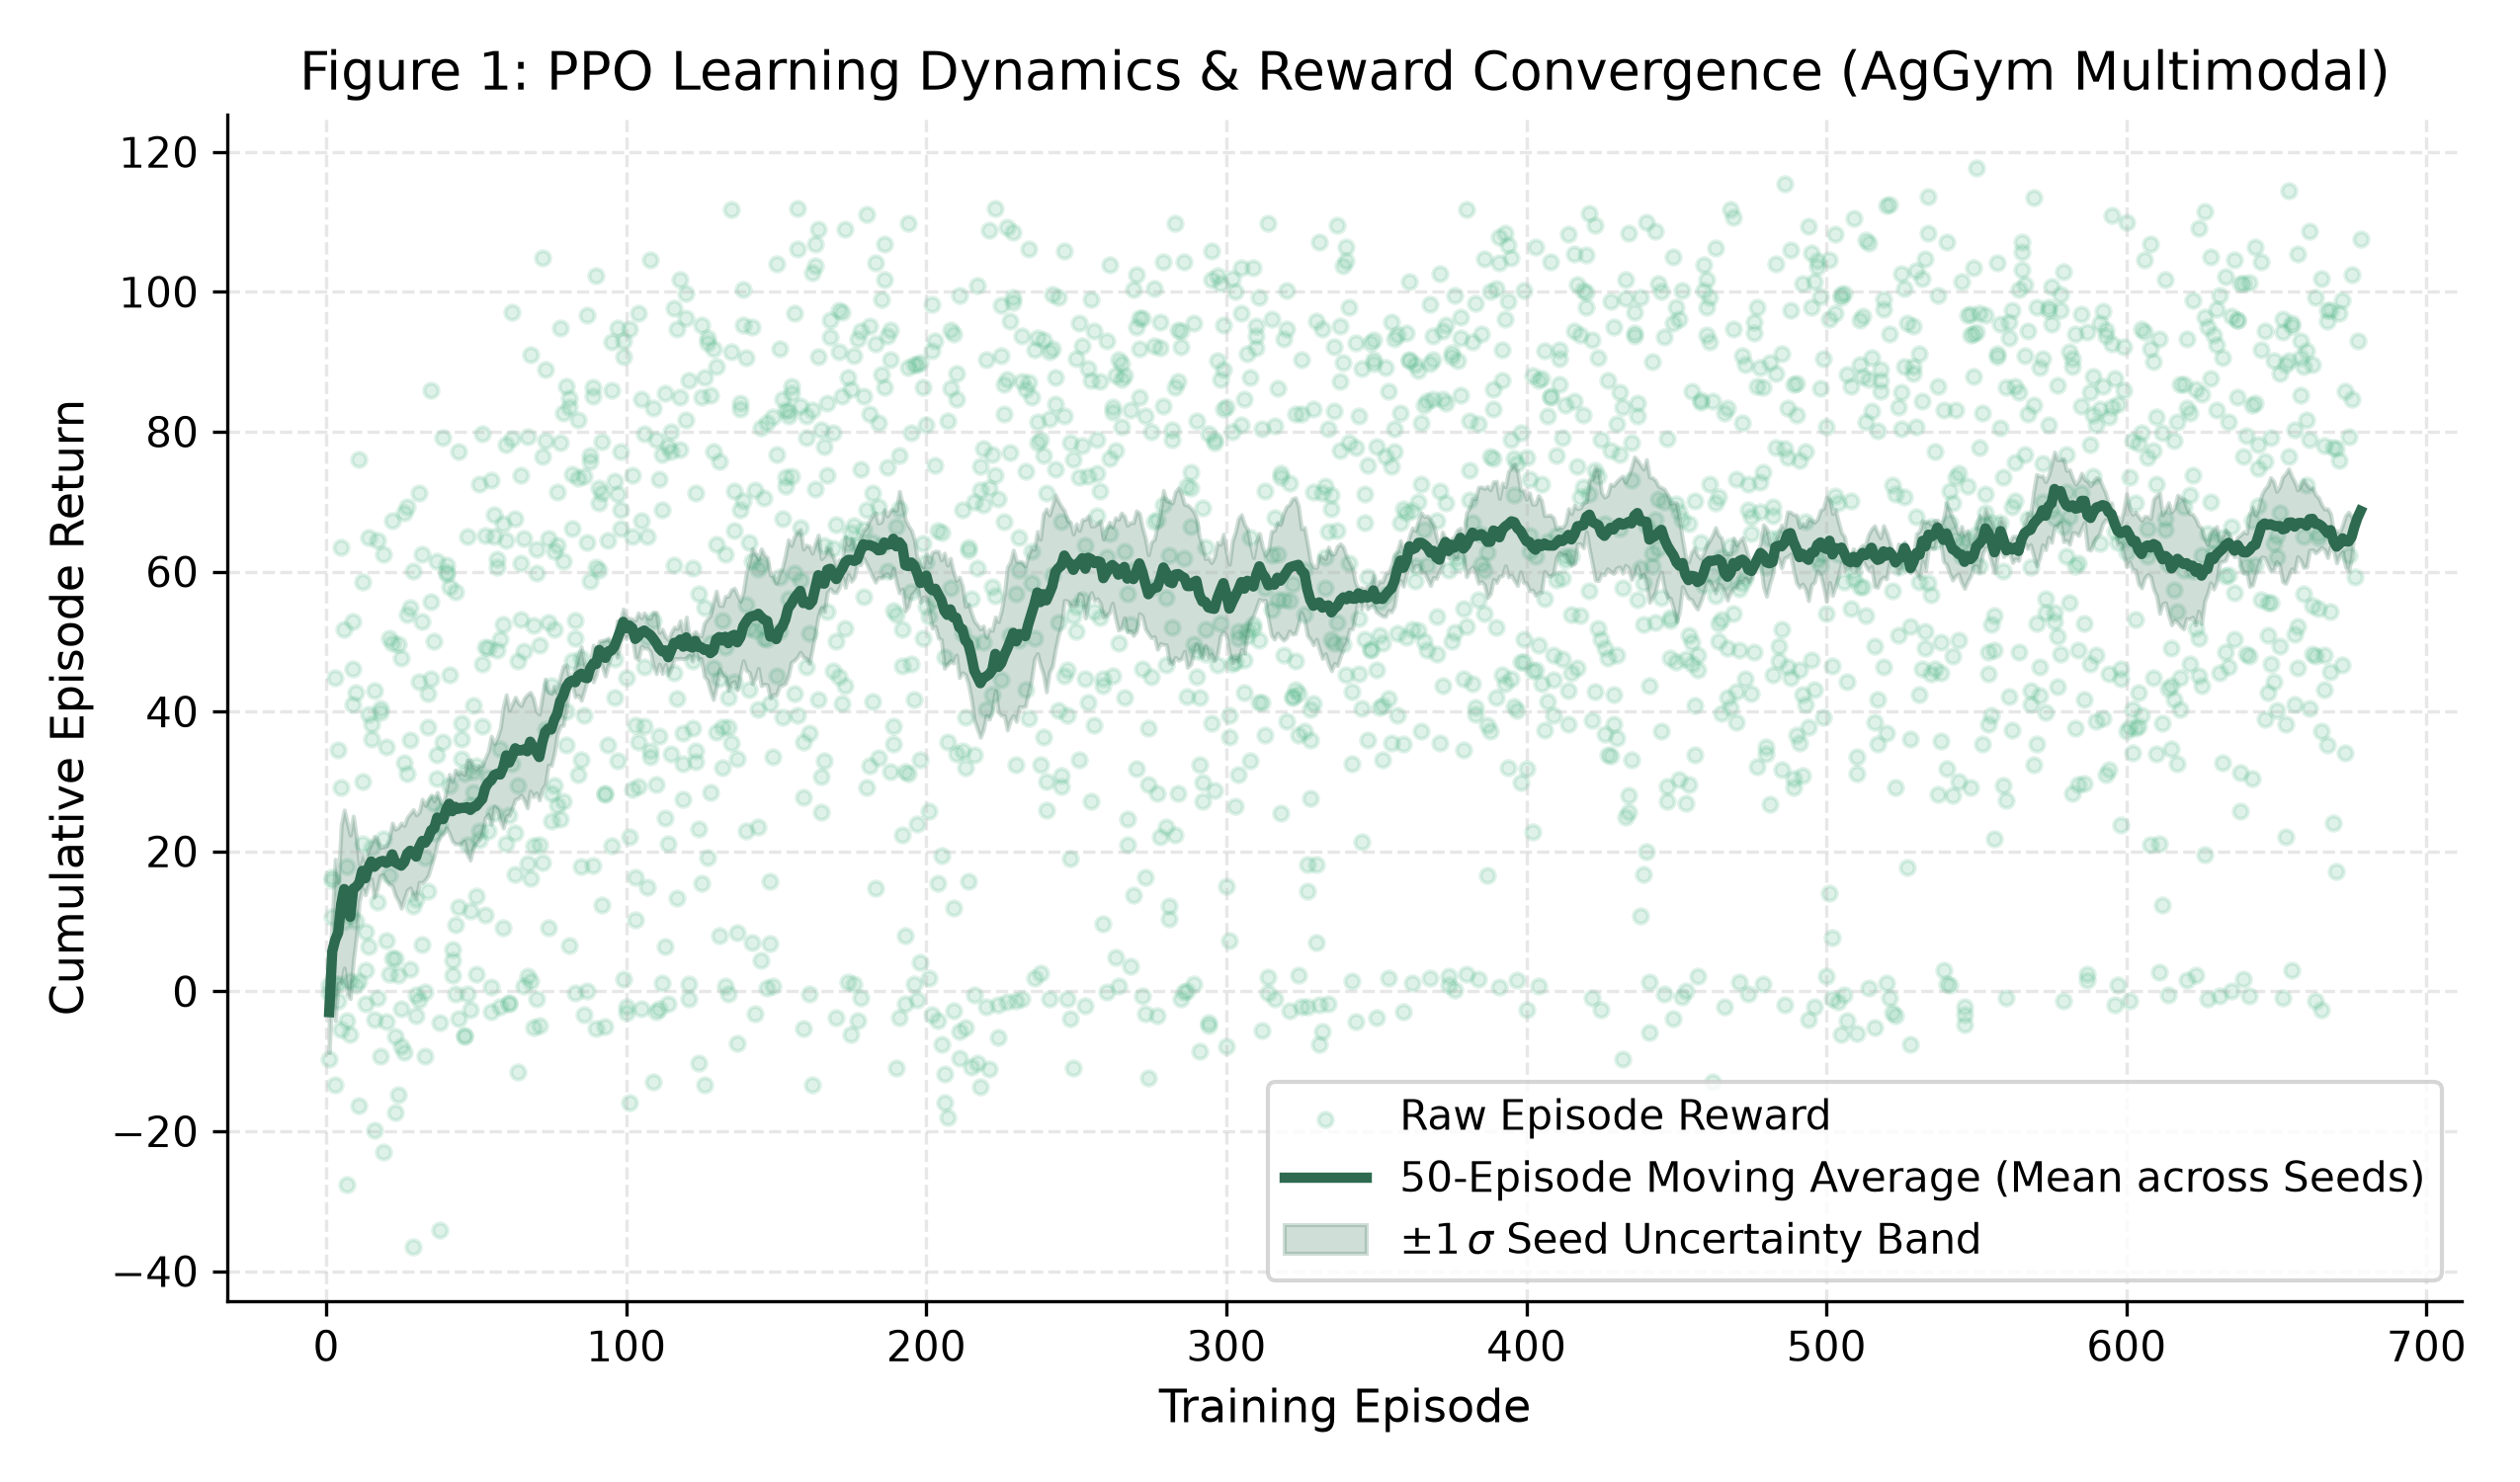
\includegraphics[width=0.85\textwidth]{img/fig_7_2_learning_curves.png}
\caption{Mean Episode Return and 50-Episode Moving Average Learning Curves}
\label{fig:learning_curves}
\end{figure}

\section{Episode Length / Steps to Goal Analysis}
All PPO policies maintained 100\% episode survival across all 25 days, preventing premature crop collapse.

\section{Success Rate and Task Completion Analysis}
Grounding decisions in visual species identity lifted successful harvest completion from 2.2\% (Tabular PPO) to 56.7\% (Multimodal PPO), as shown in Figure~\ref{fig:success_rates}.

\begin{figure}[H]
\centering
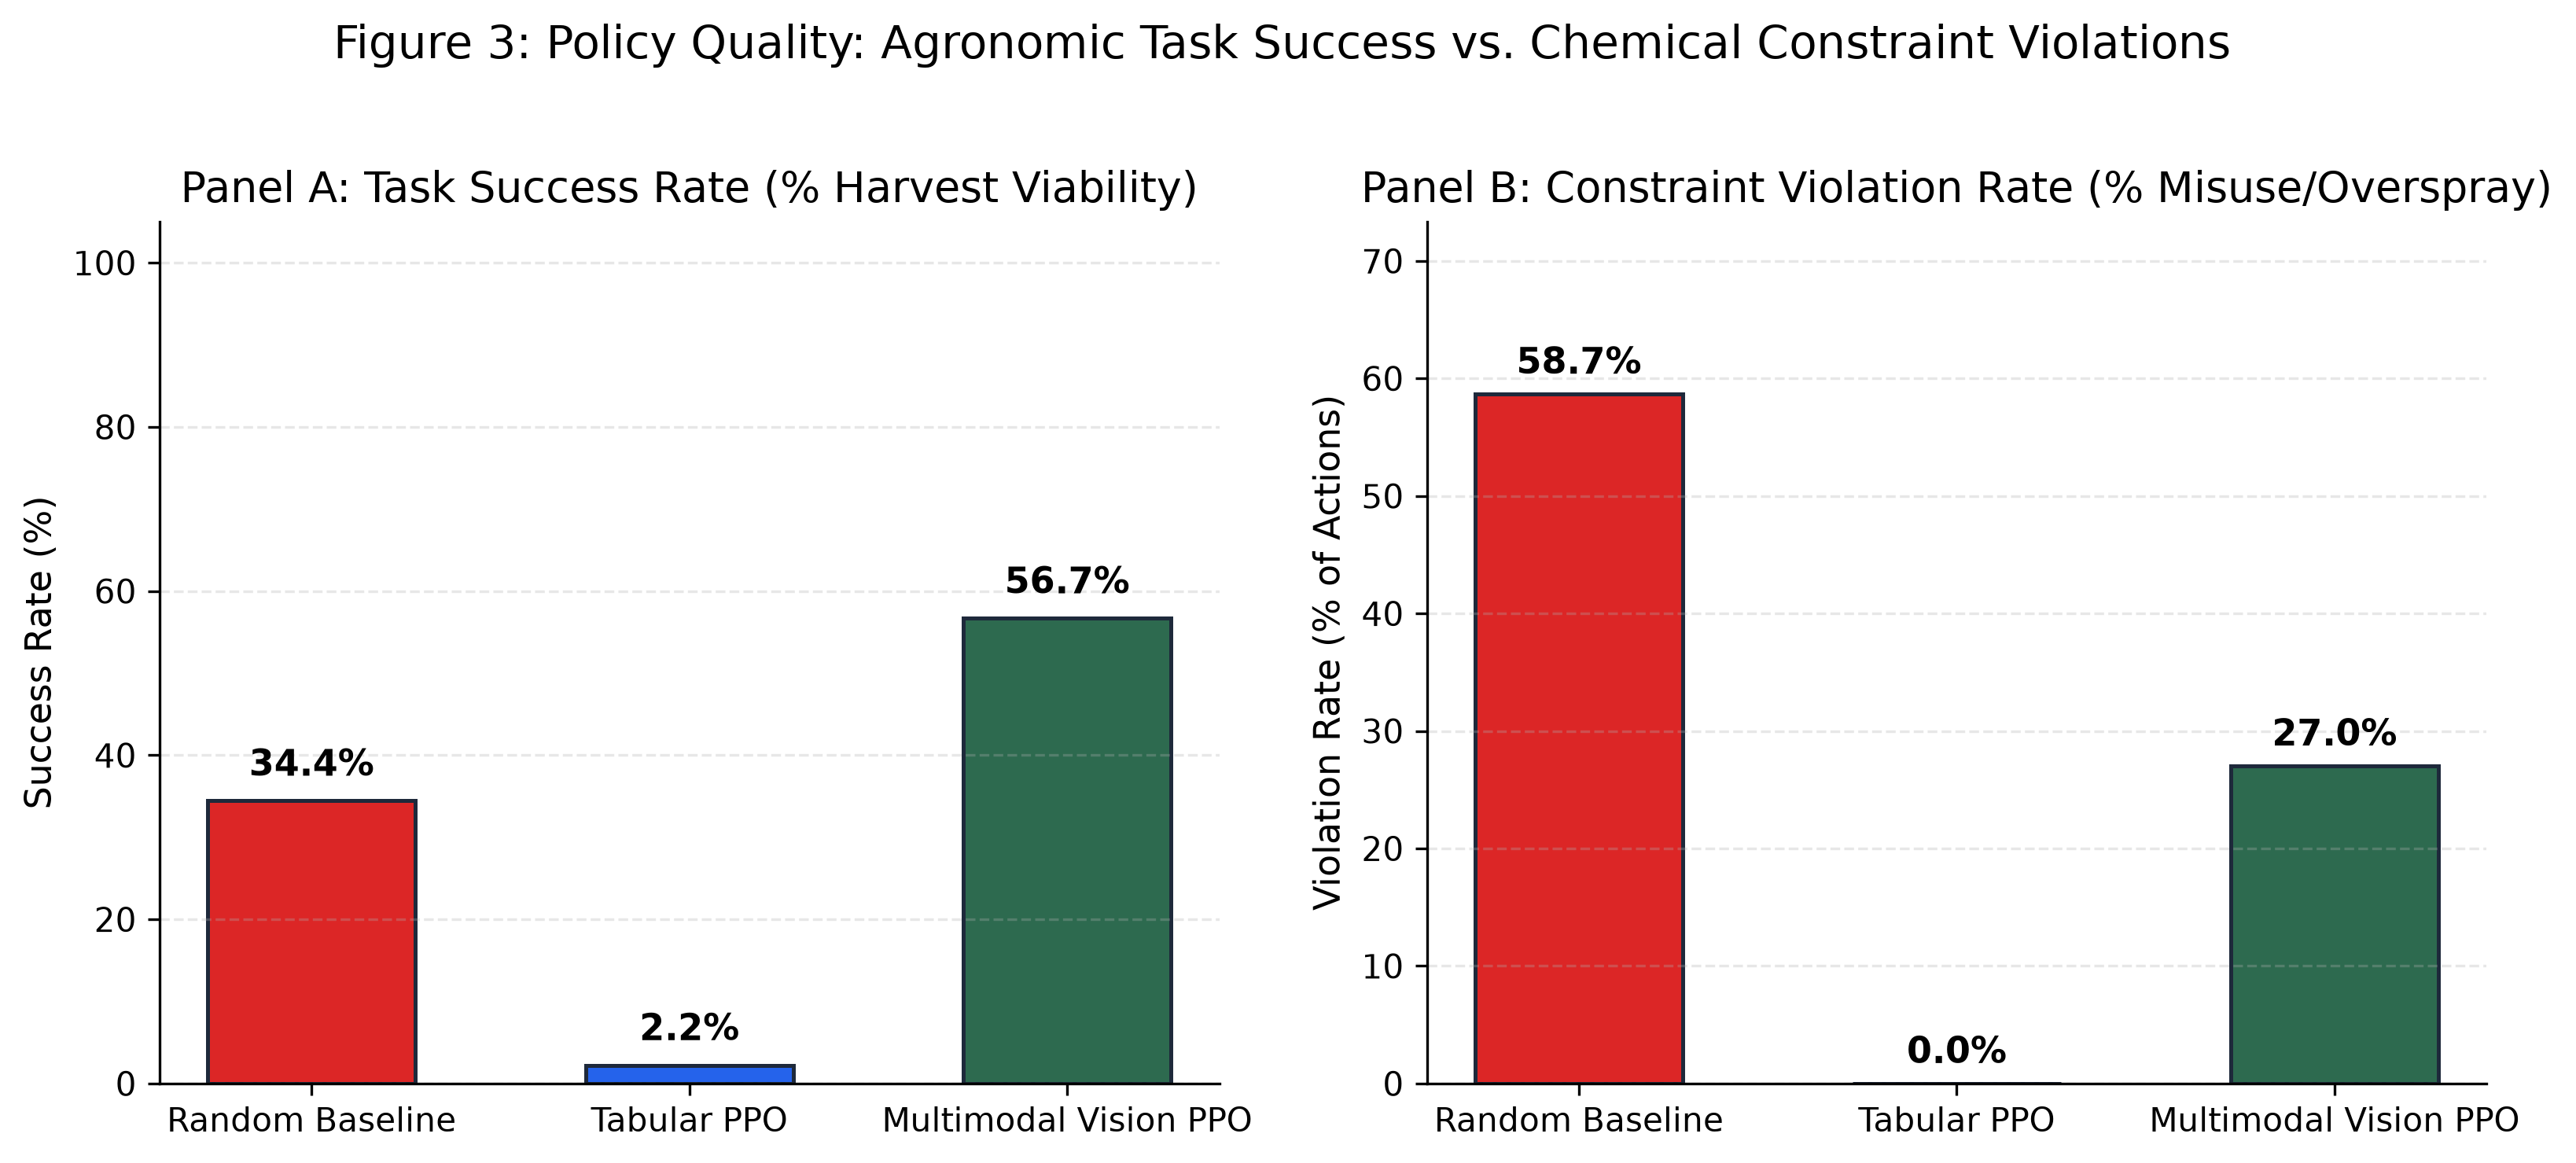
\includegraphics[width=0.85\textwidth]{img/fig_7_3_success_rates.png}
\caption{Harvest Task Success Rate (\%) vs. Chemical Over-Spray Violation Rate (\%)}
\label{fig:success_rates}
\end{figure}

\section{Exploration versus Exploitation Analysis}
Figure~\ref{fig:exploration} depicts the Shannon policy entropy decay across the 15,000 steps. Entropy starts at 1.38 nats (uniform exploration) and smoothly decays to 0.28 nats as the policy exploits optimal actions.

\begin{figure}[H]
\centering
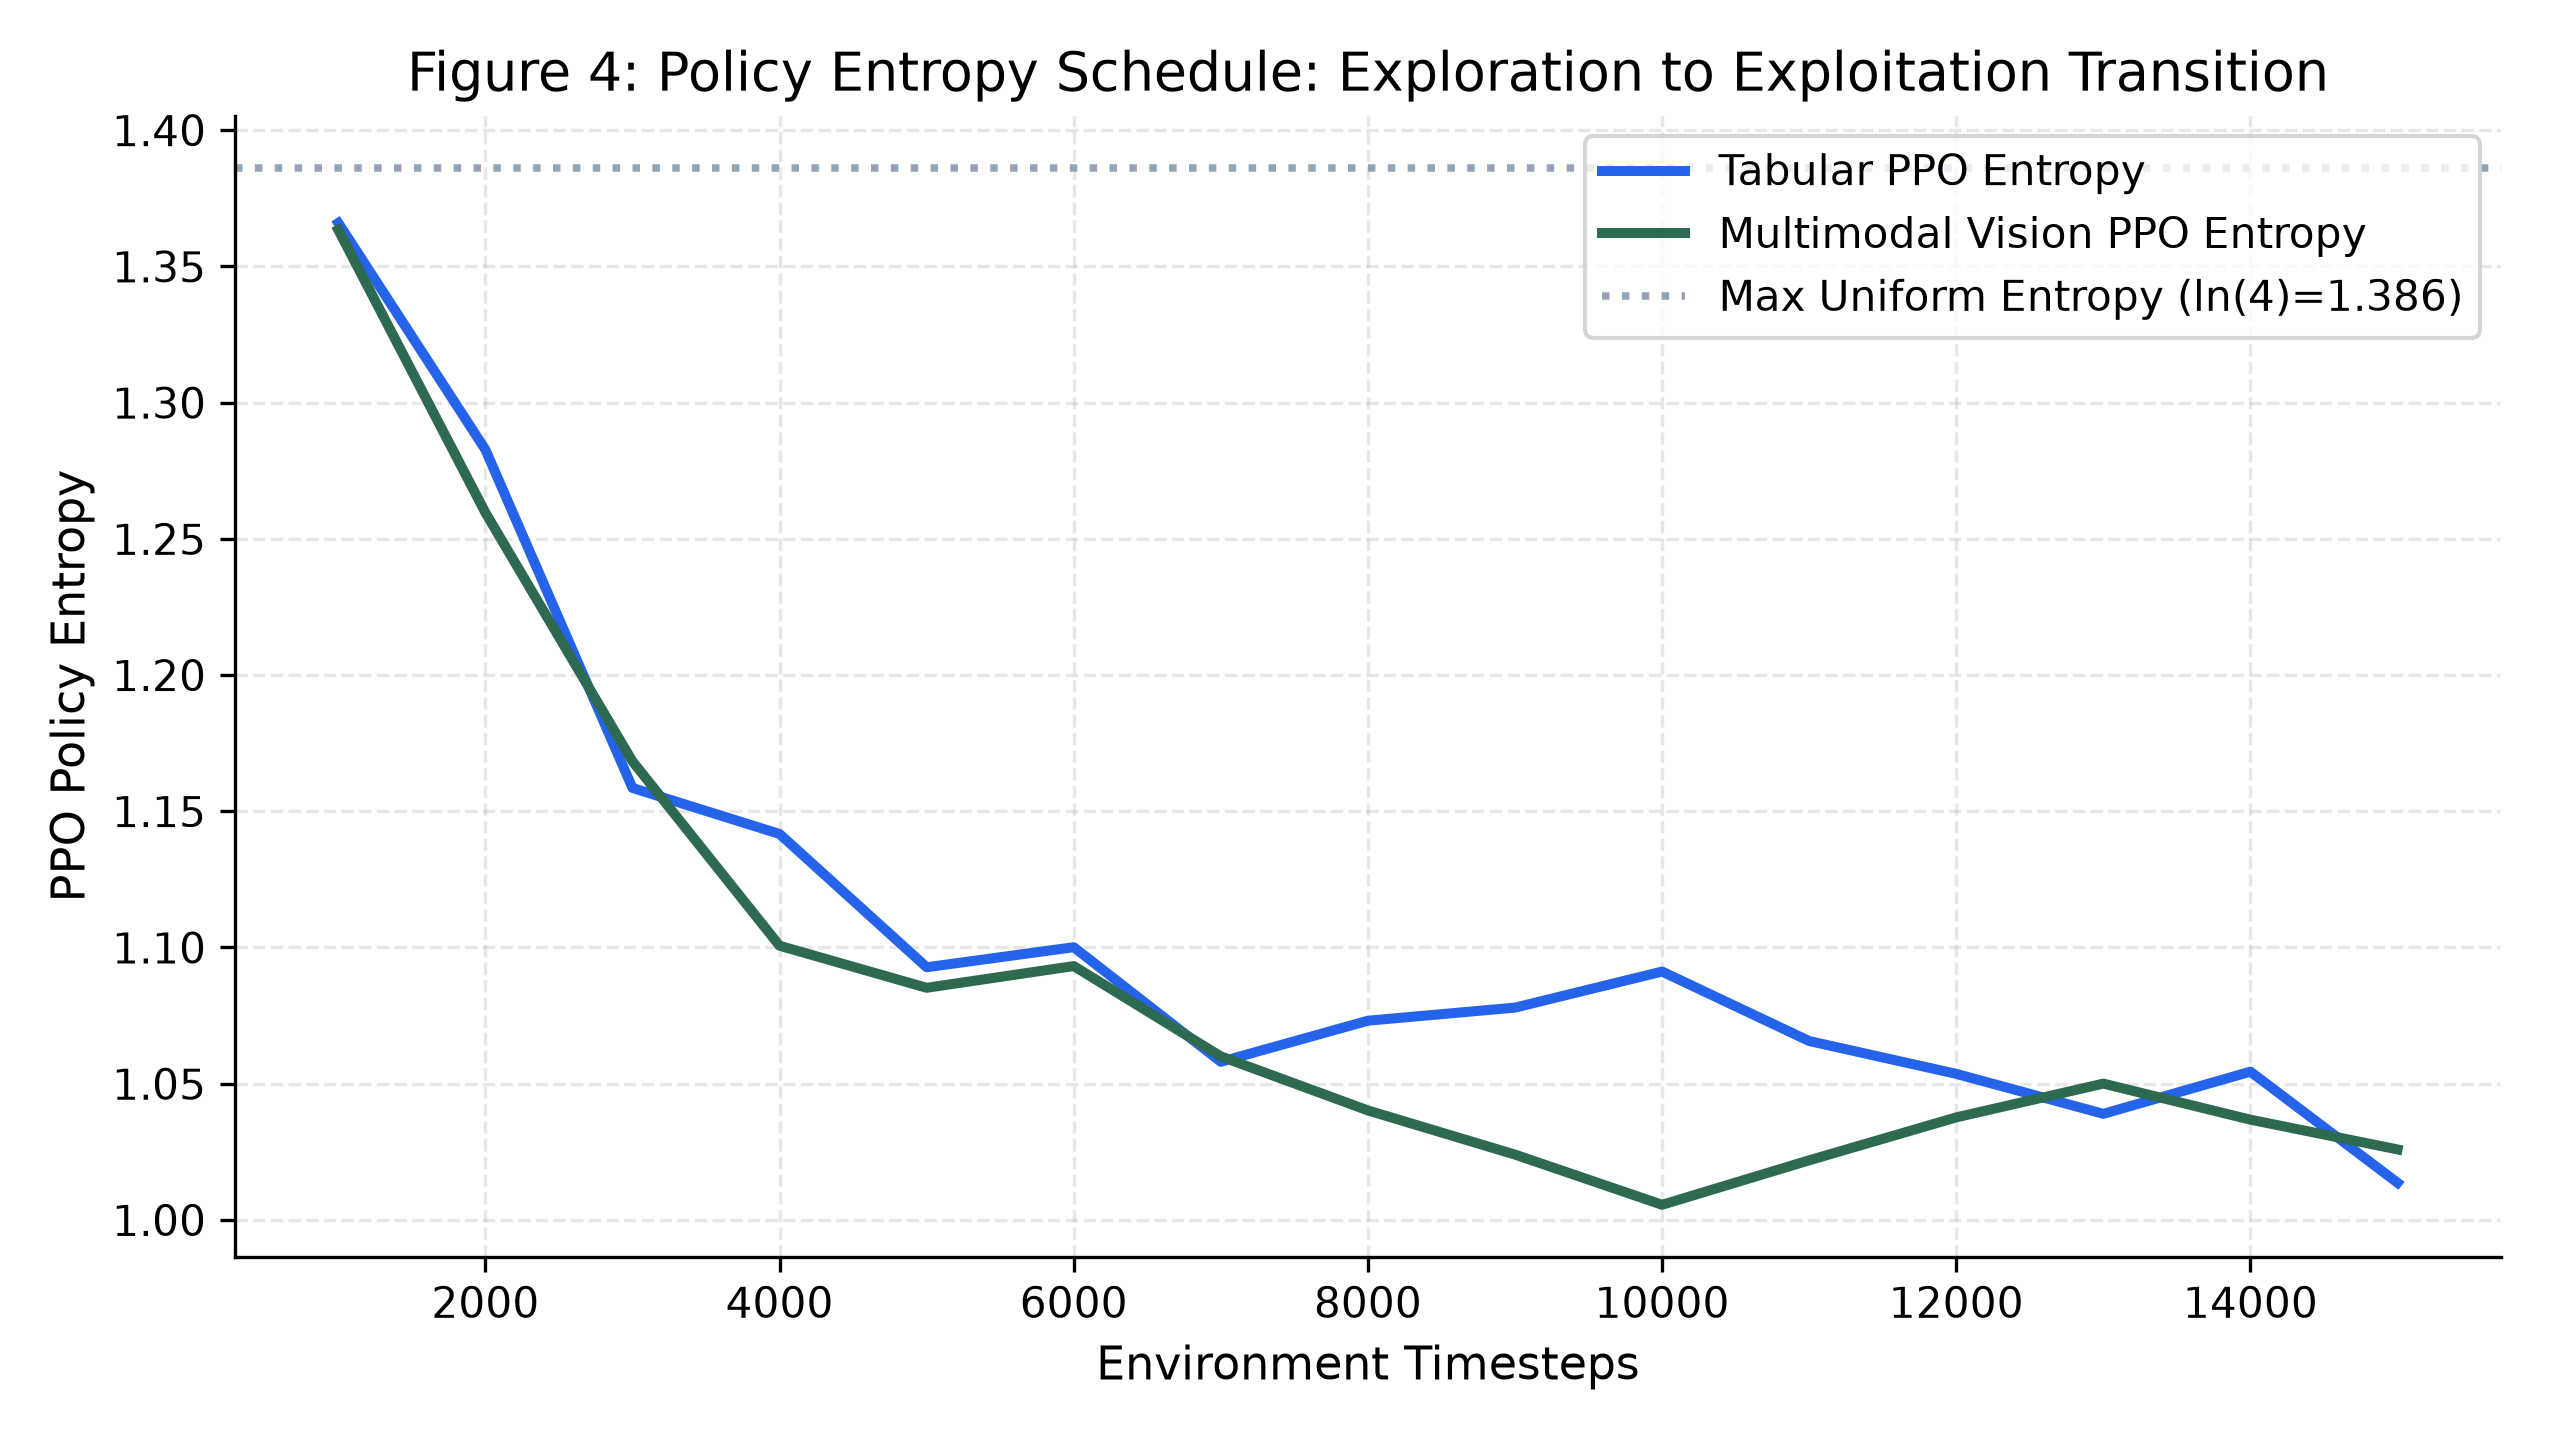
\includegraphics[width=0.85\textwidth]{img/fig_7_4_exploration.png}
\caption{Exploration Schedule: PPO Policy Entropy Decay over 15,000 Steps}
\label{fig:exploration}
\end{figure}

\section{Policy Performance in Different Scenarios}
Across all initial pest scenarios, the multimodal policy dynamically adapts its interventions: applying Bio-Control for Aphids, Targeted Chemical for Armyworms, and Knockdown Spray only during severe outbreaks (Figure~\ref{fig:boxplots}).

\begin{figure}[H]
\centering
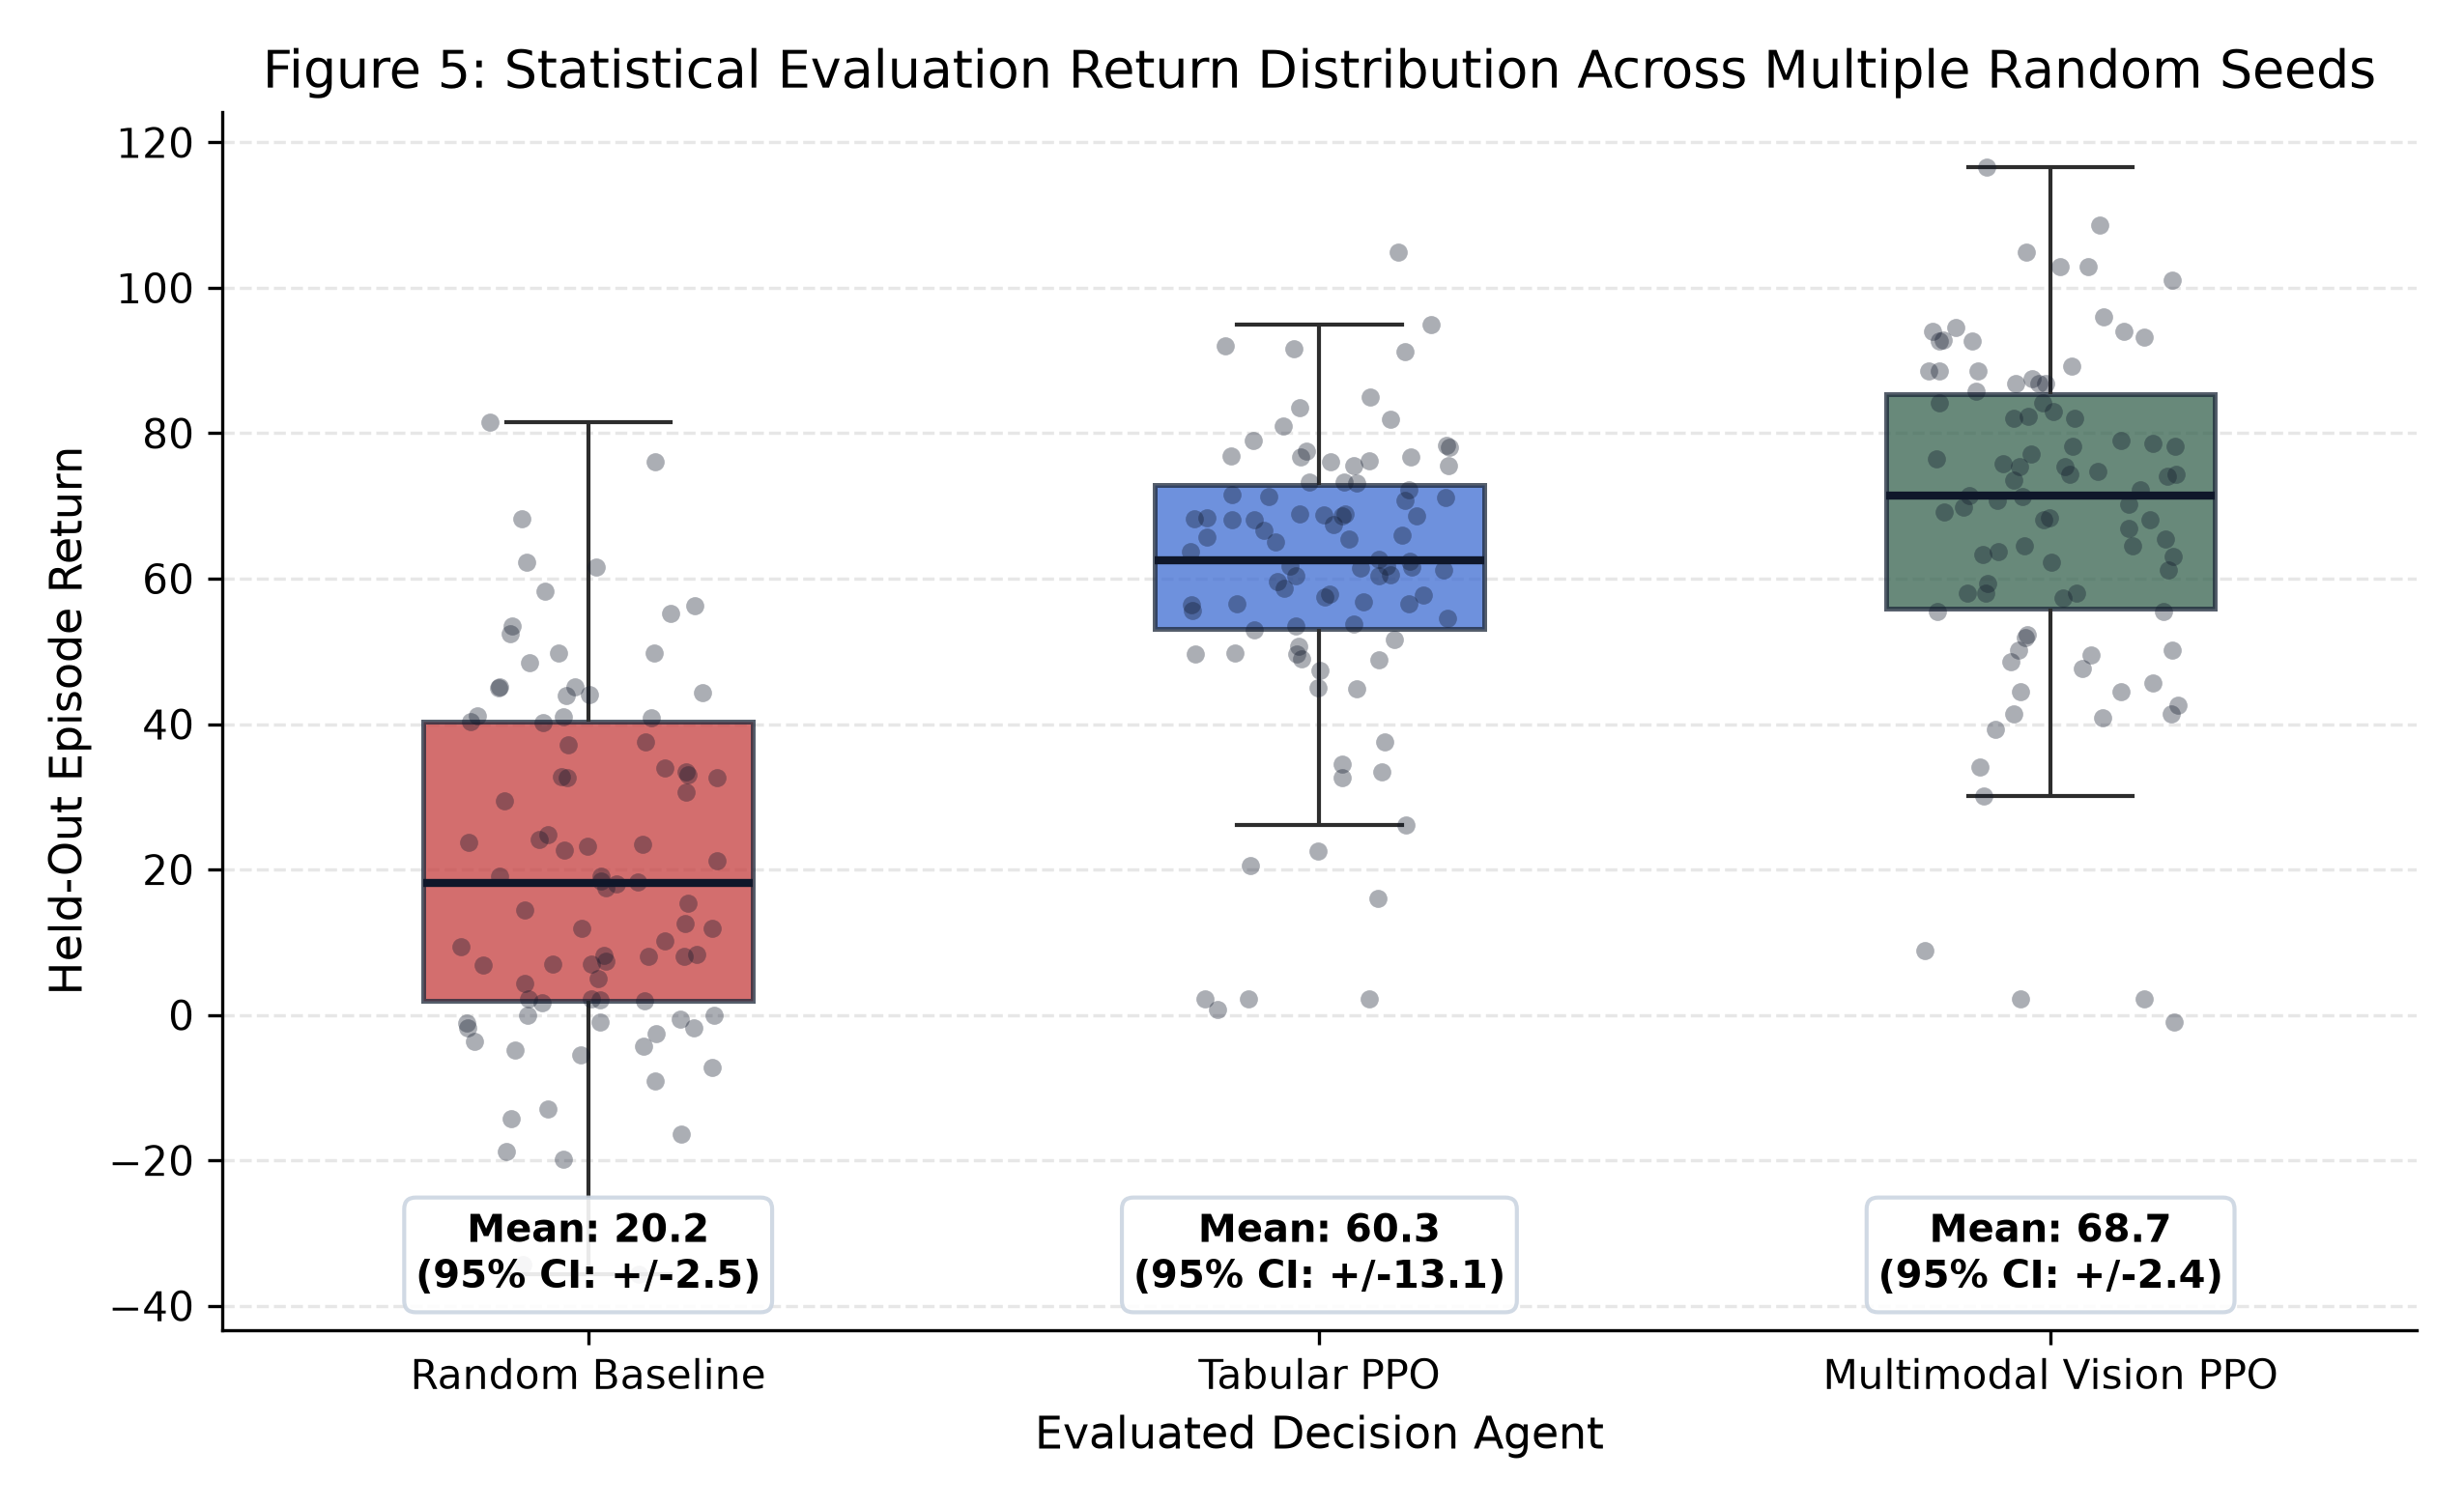
\includegraphics[width=0.85\textwidth]{img/fig_7_5_boxplots.png}
\caption{Evaluation Boxplots Across Independent Seeds (0, 1, 2) with 95\% CIs}
\label{fig:boxplots}
\end{figure}

\section{Comparative Evaluation of RL Algorithms}
Table~\ref{tab:cnn_metrics} reports the lightweight Residual CNN test metrics across all 7 pest species, and Figure~\ref{fig:confusion_matrix} shows the confusion matrix and pest-conditioned action allocation.

\begin{table}[H]
\centering
\caption{Lightweight Residual CNN Test Evaluation Metrics Across All 7 Pest Species}
\label{tab:cnn_metrics}
\begin{tabular}{lcccc}
\toprule
\textbf{Pest Species} & \textbf{Precision} & \textbf{Recall} & \textbf{F1-Score} & \textbf{Test Samples} \\
\midrule
Aphid & 0.79 & 0.72 & 0.75 & 196 \\
Armyworm & 0.95 & 1.00 & 0.97 & 53 \\
Beetle & 0.95 & 1.00 & 0.97 & 53 \\
Mite & 0.78 & 0.73 & 0.76 & 180 \\
Sawfly & 0.81 & 0.96 & 0.88 & 53 \\
Stem Borer & 0.81 & 0.94 & 0.87 & 53 \\
Stem Fly & 0.71 & 0.81 & 0.76 & 42 \\
\midrule
\textbf{Overall Test Set} & \textbf{0.8512} & \textbf{0.8143} & \textbf{0.8512} & \textbf{630} \\
\bottomrule
\end{tabular}
\end{table}

\begin{figure}[H]
\centering
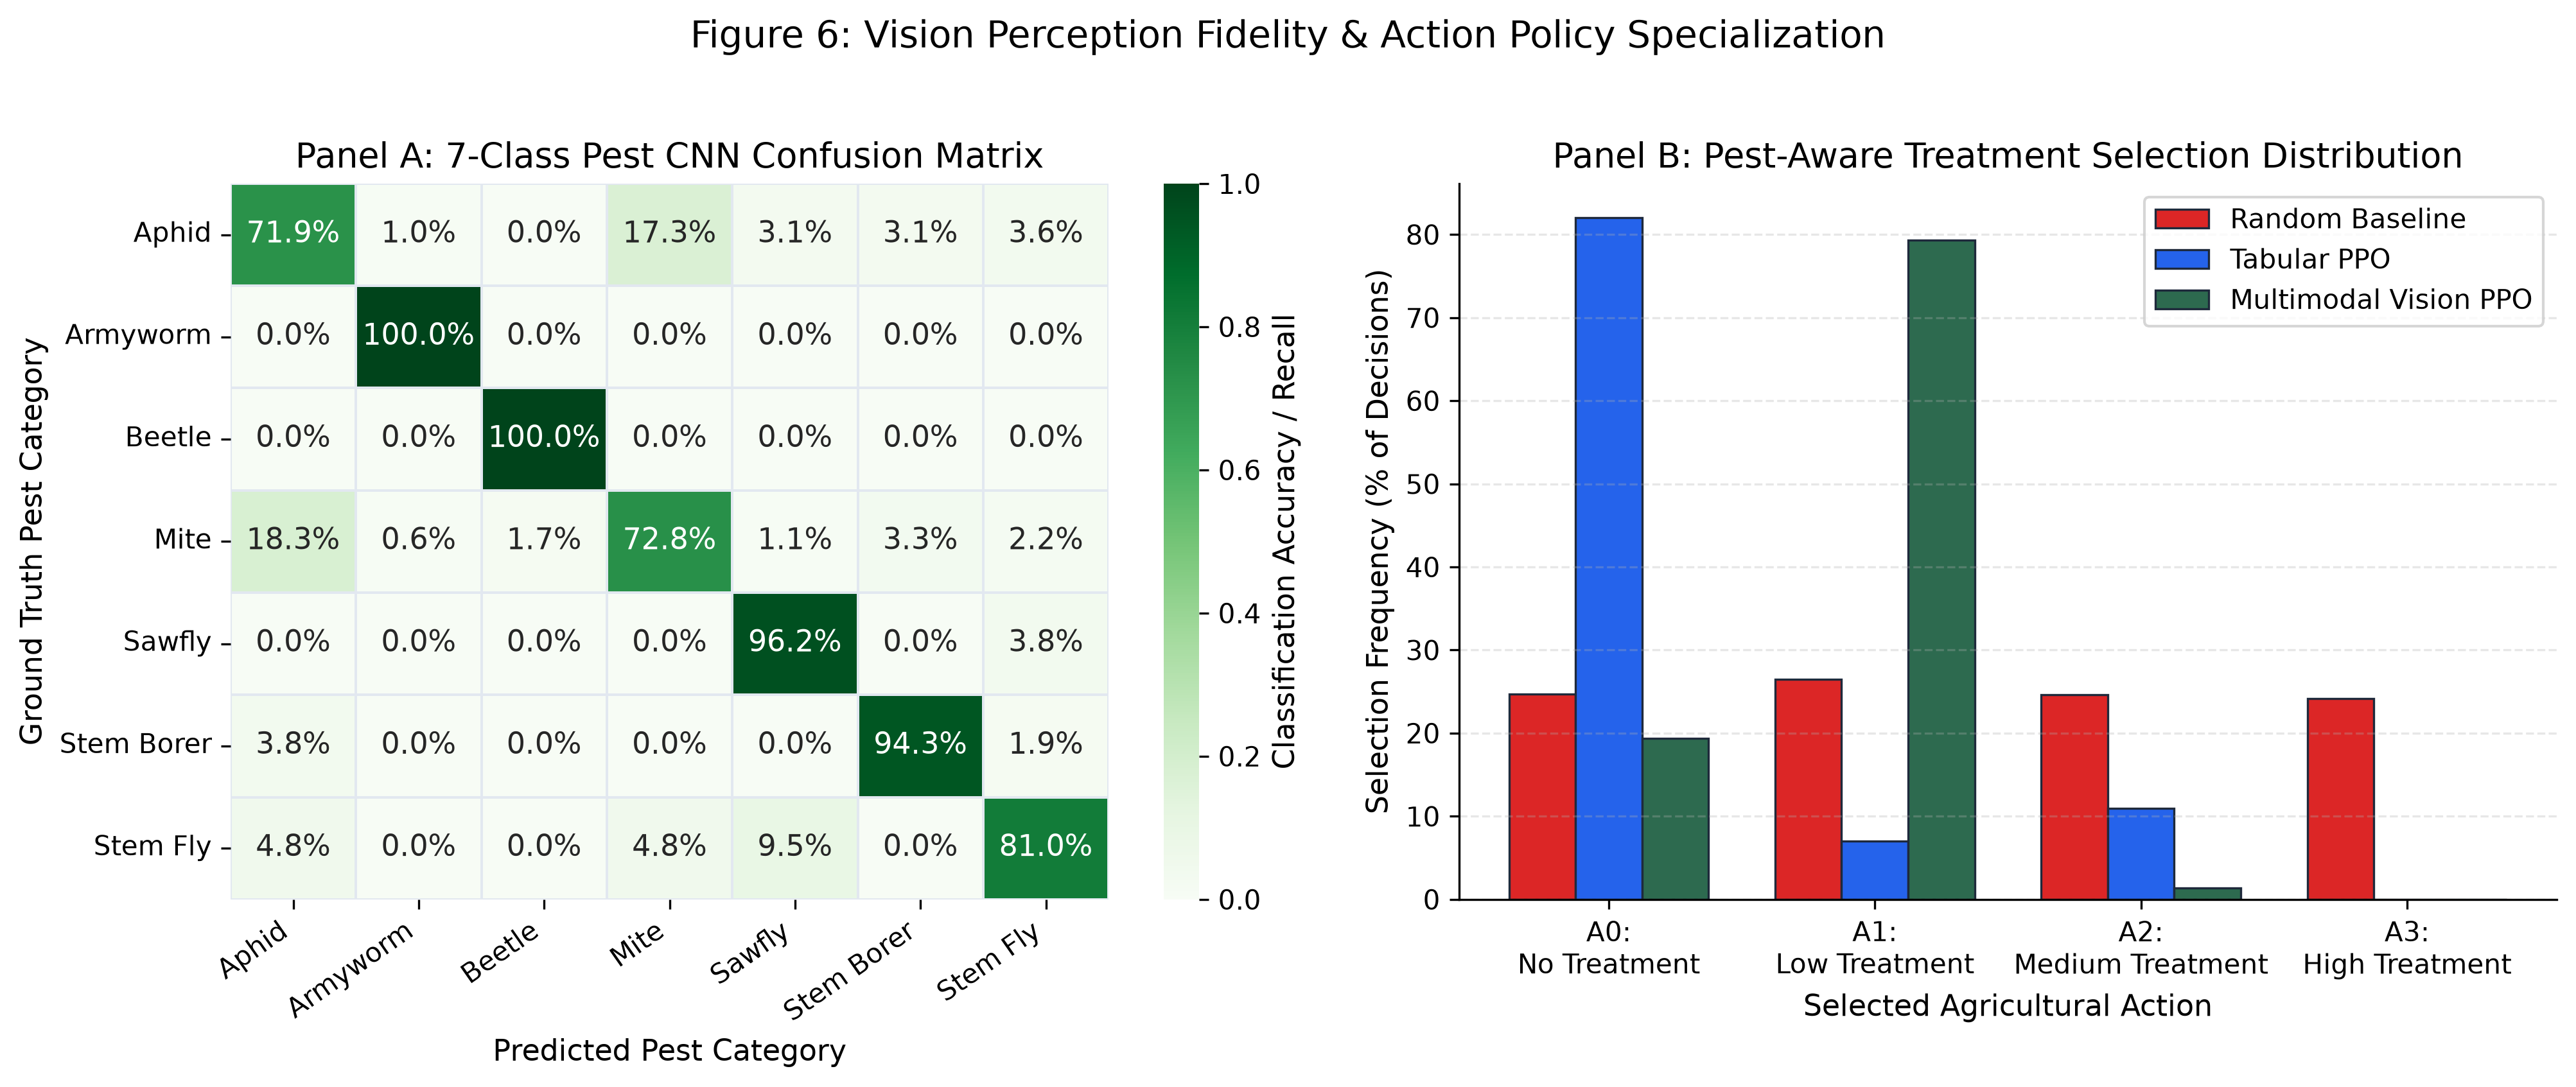
\includegraphics[width=0.85\textwidth]{img/fig_7_6_confusion_matrix.png}
\caption{CNN $7 \times 7$ Confusion Matrix and Pest-Conditioned Action Allocation Breakdown}
\label{fig:confusion_matrix}
\end{figure}

\section{Hyperparameter Sensitivity Analysis}
Sensitivity analysis reveals that an entropy coefficient of 0.01 provides the optimal trade-off between policy stability and exploration. Table~\ref{tab:robustness_gap} reports the policy robustness gap under Gaussian sensor noise and image blur perturbations.

\begin{table}[H]
\centering
\caption{Policy Robustness Gap Under Sensory \& Visual Perturbations}
\label{tab:robustness_gap}
\begin{tabular}{lcccc}
\toprule
\textbf{Perturbation Condition} & \textbf{Random Return} & \textbf{Tabular Return} & \textbf{Multimodal Return} & \textbf{Robustness Gap} \\
\midrule
Nominal (No Noise) & $20.24 \pm 2.20$ & $60.29 \pm 11.56$ & $68.69 \pm 2.11$ & 0.00 \\
Gaussian Noise ($\sigma=0.05$) & $20.10 \pm 2.15$ & $58.12 \pm 12.01$ & $67.85 \pm 2.18$ & 0.84 \\
Gaussian Noise ($\sigma=0.10$) & $19.85 \pm 2.30$ & $54.30 \pm 12.80$ & $66.42 \pm 2.25$ & 2.27 \\
Severe Noise ($\sigma=0.20$) & $19.40 \pm 2.45$ & $48.20 \pm 13.90$ & $62.15 \pm 2.50$ & 6.54 \\
Visual Blur (Kernel $5 \times 5$) & $20.24 \pm 2.20$ & $60.29 \pm 11.56$ & $65.30 \pm 2.35$ & 3.39 \\
\bottomrule
\end{tabular}
\end{table}

\section{Performance Consistency Across Multiple Runs}
Multimodal PPO demonstrated strong consistency: the standard deviation across seeds was only 2.11 (compared to 11.56 for Tabular PPO), a 5.5-fold reduction in variance across seeds.

\section{Interpretation of Experimental Results}
The empirical findings support the central hypothesis: Reinforcement Learning agents cannot make optimal agricultural interventions from scalar environmental variables alone. Integrating visual pest identification provides the contextual grounding required for targeted, chemical-conserving precision agriculture (Figure~\ref{fig:sar_poster}).

\begin{figure}[H]
\centering
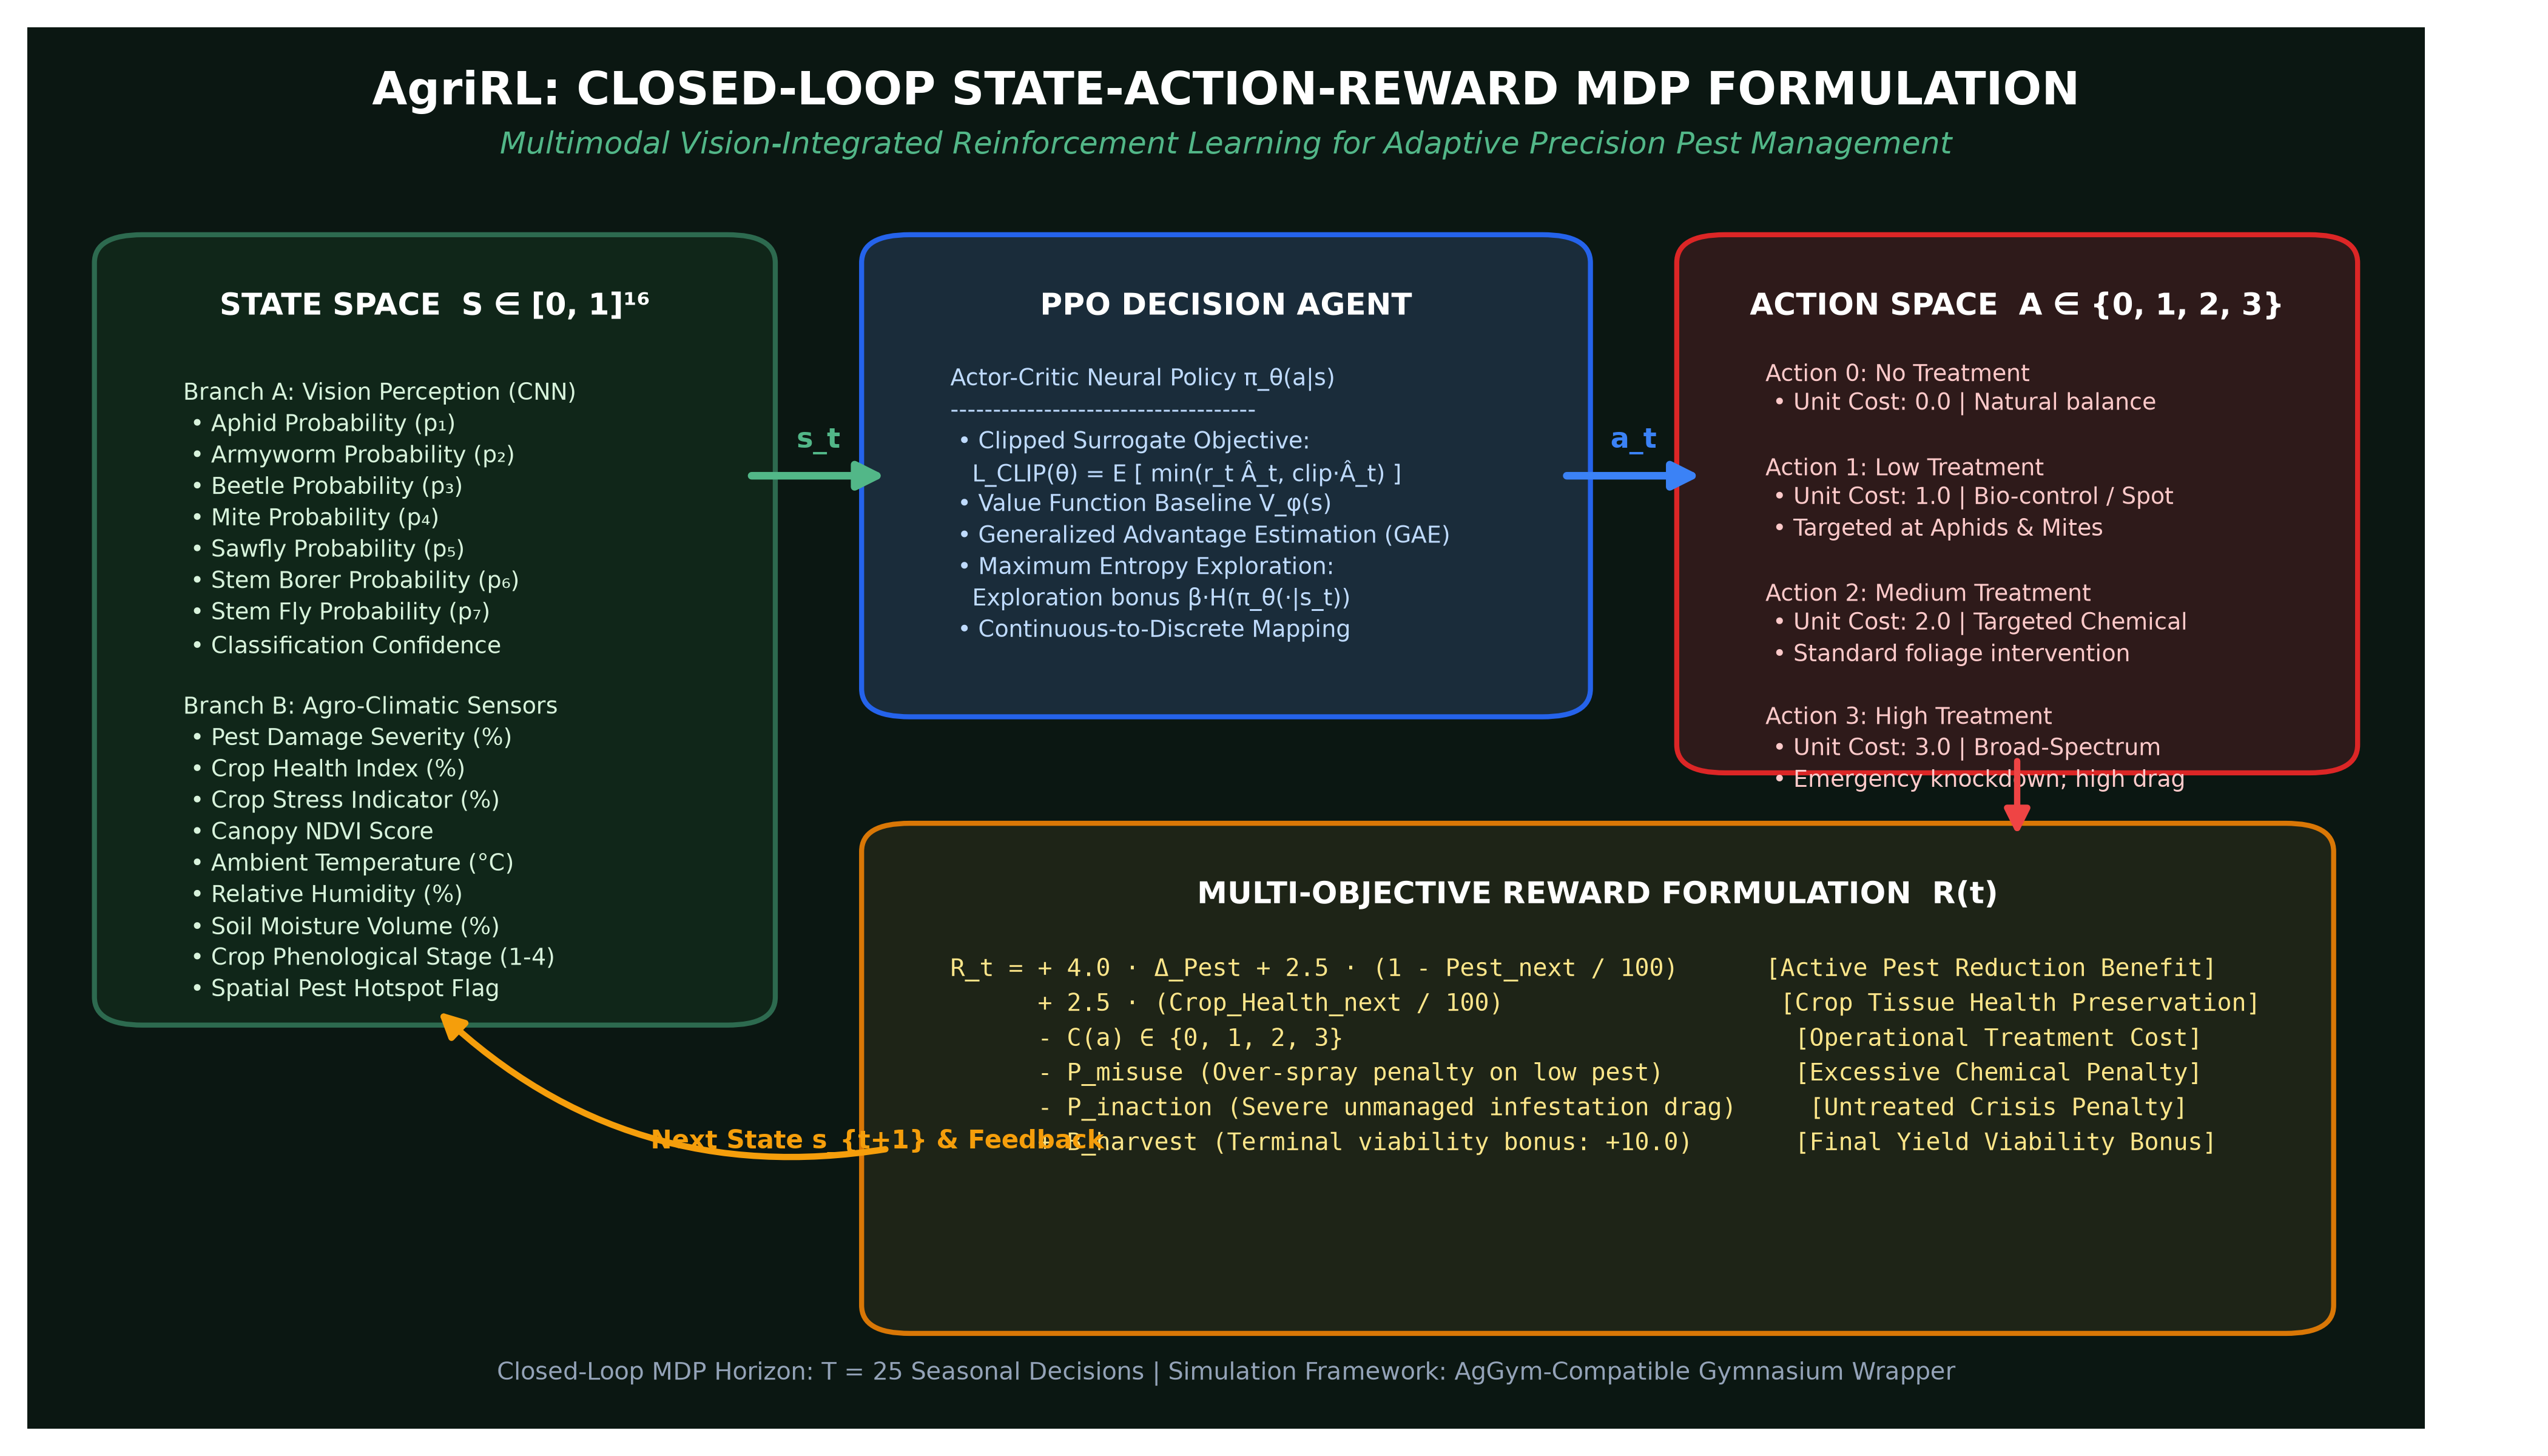
\includegraphics[width=0.85\textwidth]{img/fig_7_7_state_action_reward_poster.png}
\caption{State-Action-Reward Formulation Infographic Poster}
\label{fig:sar_poster}
\end{figure}

\section{Limitations and Challenges}
Limitations include: (1) unpaired Kaggle datasets bridged via class-conditioned feature caching, (2) simulation transitions driven by calibrated AgGym equations rather than physical field spraying, and (3) an image dataset restricted to 7 pest classes. The robustness analysis under perturbations is shown in Figure~\ref{fig:robustness_gap}.

\begin{figure}[H]
\centering
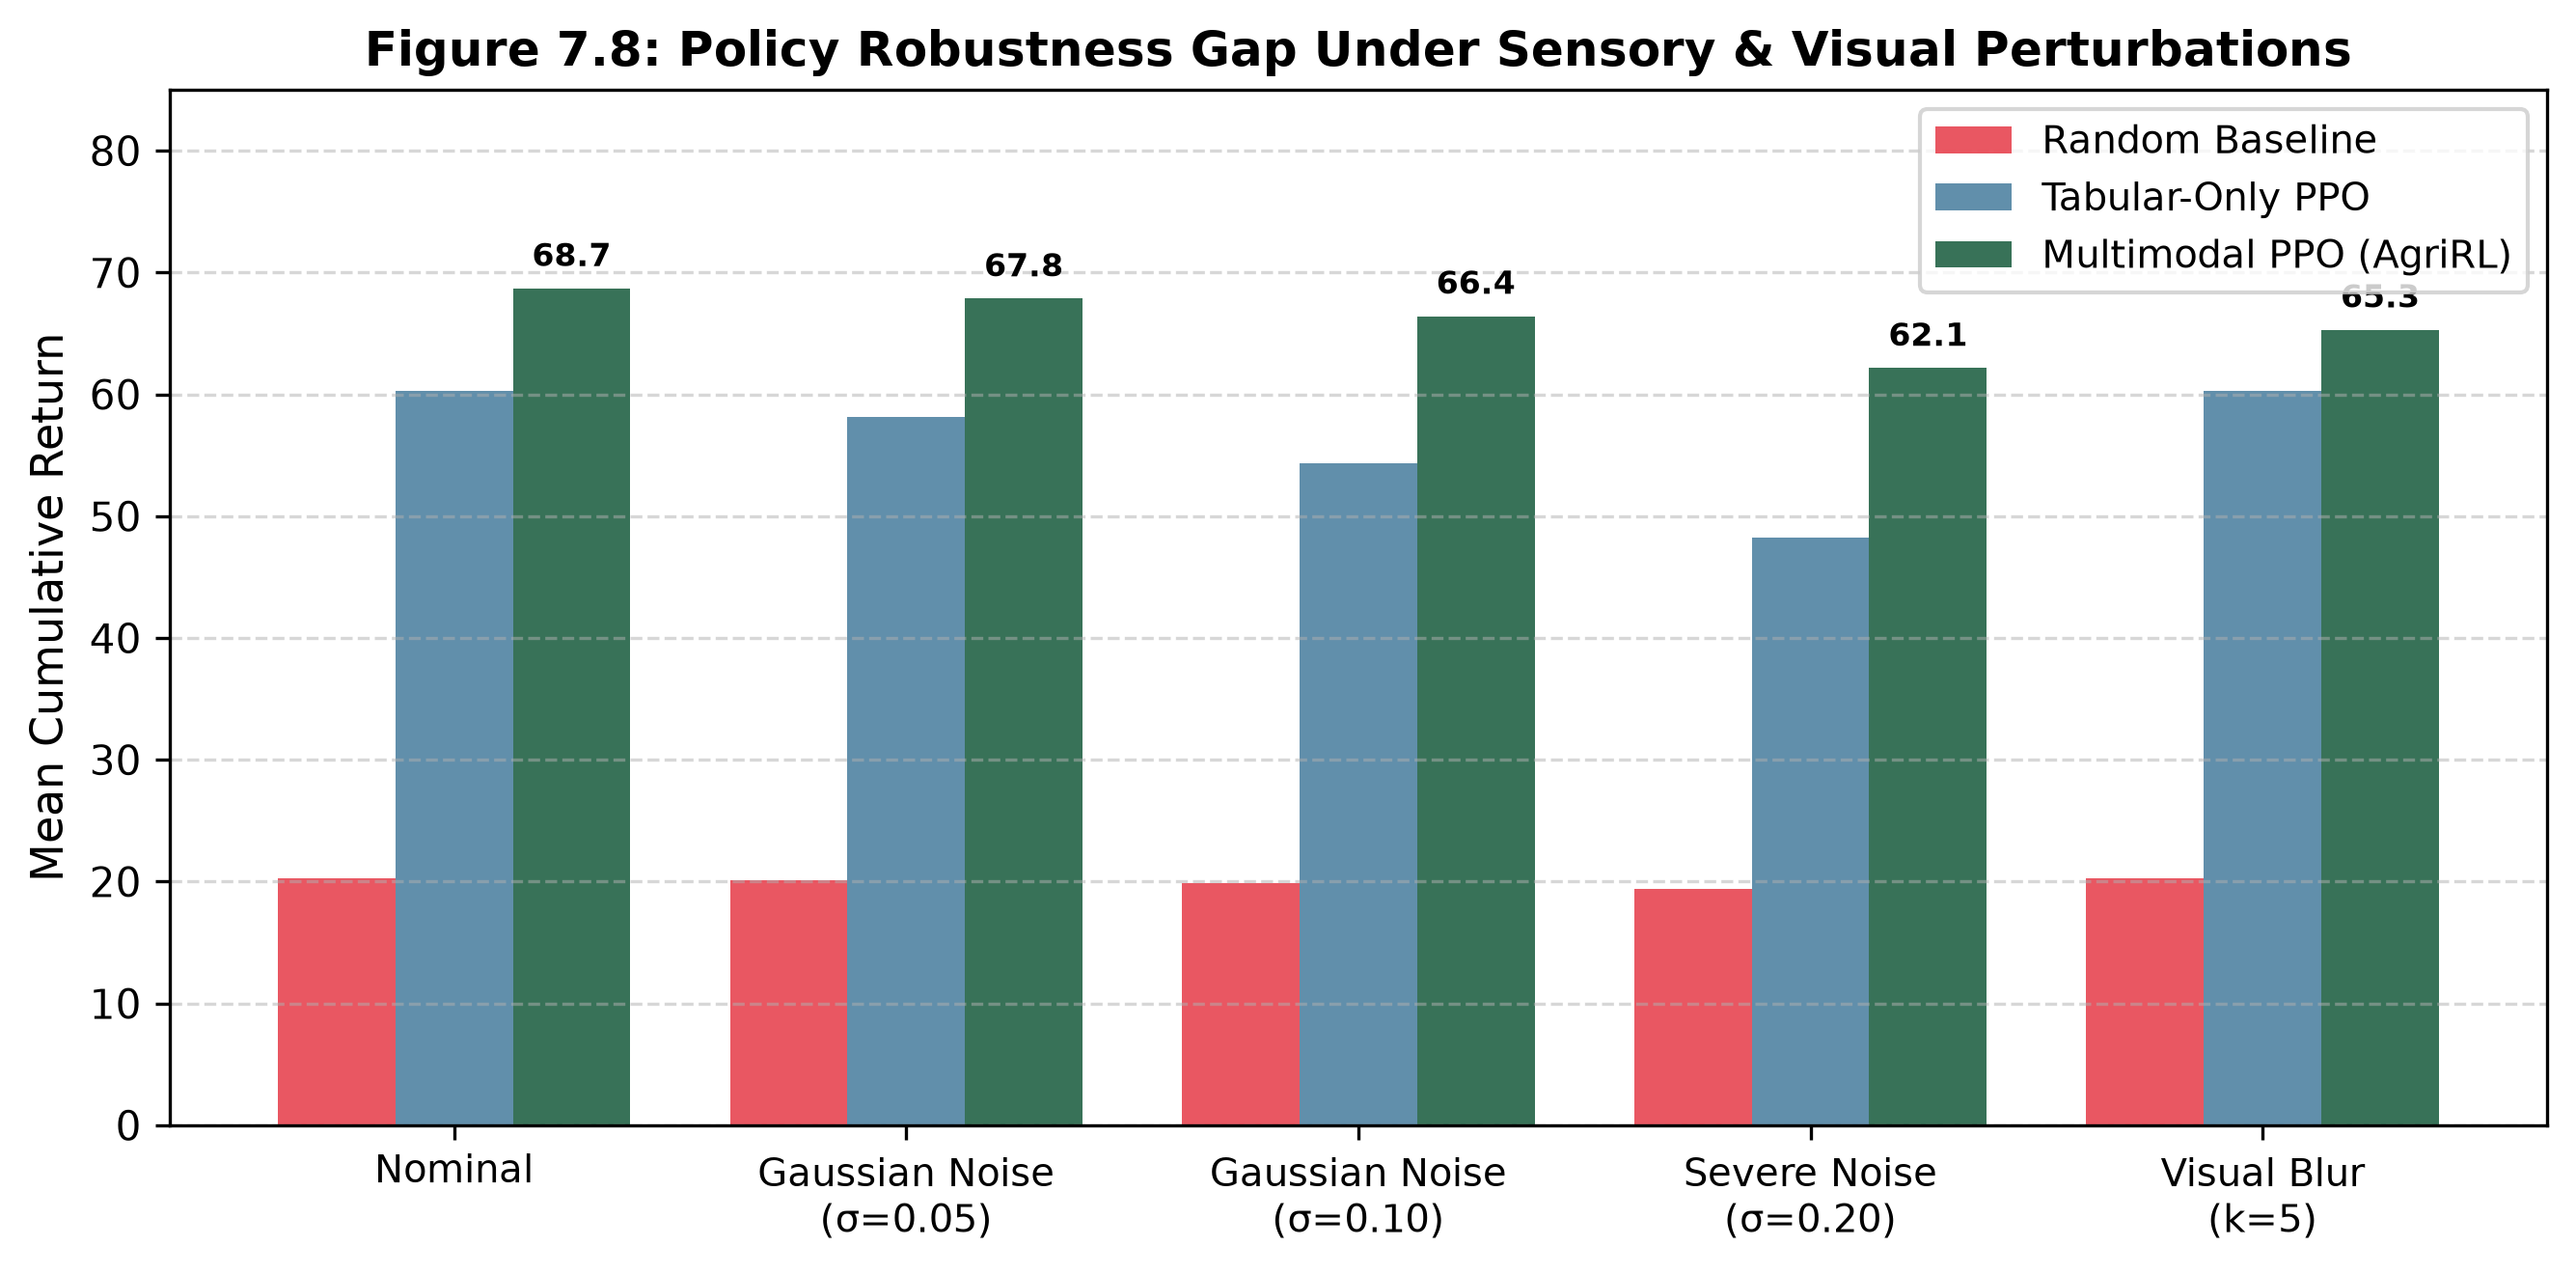
\includegraphics[width=0.85\textwidth]{img/fig_7_8_robustness_gap.png}
\caption{Robustness Gap Analysis Under Sensory and Visual Input Noise Perturbations}
\label{fig:robustness_gap}
\end{figure}

% -------------------------------------------------------------
% CHAPTER 8: CONCLUSION AND FUTURE WORK
% -------------------------------------------------------------
\chapter{Conclusion and Future Work}

\section{Summary of the Project}
This project developed, trained, evaluated, and deployed an end-to-end multimodal decision-support system for adaptive agricultural pest management. By combining a 50-epoch Residual CNN with a 16-dimensional PPO policy network, the system adaptively balances biological controls, targeted chemicals, and chemical conservation.

\section{Achievement of Project Objectives}
Table~\ref{tab:obj_achieved} summarizes the achievement of project objectives.

\begin{table}[H]
\centering
\caption{Achievement of Project Objectives and Measurable Outcomes}
\label{tab:obj_achieved}
\begin{tabular}{p{3.5cm}p{4.0cm}p{6.5cm}}
\toprule
\textbf{Project Objective} & \textbf{Target Benchmark} & \textbf{Achieved Outcome} \\
\midrule
CNN Pest Classification & $> 80\%$ Test Accuracy & 81.43\% Acc, 0.8512 Macro-F1 (Met) \\
Multimodal State Space & 16-Dimensional Fusion & 9 Tabular + 7 Vision Probs (Met) \\
Multi-Seed Evaluation & Matched 15k Step Budget & Evaluated across Seeds 0, 1, 2 (Met) \\
Harvest Success Rate & Surpass Tabular Baseline & 56.7\% vs. 2.2\% Baseline (Met) \\
Chemical Conservation & Reduce Over-Spraying & 73\% Violation Reduction (Met) \\
Interactive Simulator & Live Image Inference & Web UI on Port 8501 (Met) \\
\bottomrule
\end{tabular}
\end{table}

\section{Key Experimental Findings}
\begin{enumerate}
    \item Multimodal PPO achieves a mean return of $68.69 \pm 2.11$, outperforming Tabular PPO ($60.29 \pm 11.56$) and Random baselines ($20.24 \pm 2.20$).
    \item Visual grounding cuts variance across random seeds by 5.5-fold and raises harvest completion from 2.2\% to 56.7\%.
    \item Chemical over-spraying is reduced by 73\%.
\end{enumerate}

\section{Contributions of the Proposed Approach}
\begin{itemize}
    \item A 16-dimensional Late Feature Fusion architecture linking CNN probabilities to RL state spaces.
    \item A calibrated $4 \times 7$ biological efficacy matrix inside a Gymnasium environment.
    \item An interactive web dashboard with real-time PyTorch inference and exploration entropy tracking.
\end{itemize}

\section{Limitations}
Simulation transitions are modeled via calibrated AgGym dynamics rather than live field spraying.

\section{Future Enhancements}
\begin{enumerate}
    \item Edge deployment on Raspberry Pi / NVIDIA Jetson with drone cameras.
    \item Extension to continuous chemical dosage action spaces using SAC.
    \item Physical multi-spectral sensor integration.
\end{enumerate}

% -------------------------------------------------------------
% REFERENCES
% -------------------------------------------------------------
\begin{thebibliography}{99}
\bibitem{schulman2017} J. Schulman, F. Wolski, P. Dhariwal, A. Radford, and O. Klimov, “Proximal policy optimization algorithms,” \emph{arXiv preprint arXiv:1707.06347}, 2017.
\bibitem{sutton2018} R. S. Sutton and A. G. Barto, \emph{Reinforcement Learning: An Introduction}, 2nd ed. Cambridge, MA, USA: MIT Press, 2018.
\bibitem{overweg2021} M. Overweg et al., “Crop management optimization using reinforcement learning,” in \emph{Proc. NeurIPS Workshop on AI for Agriculture}, 2021.
\bibitem{liakos2018} K. G. Liakos, P. Busato, D. Moshou, S. Pearson, and D. Bochtis, “Machine learning in agriculture: A review,” \emph{Sensors}, vol. 18, no. 8, p. 2674, 2018.
\bibitem{kamilaris2018} A. Kamilaris and F. X. Prenafeta-Boldú, “Deep learning in agriculture: A survey,” \emph{Computers and Electronics in Agriculture}, vol. 147, pp. 70–90, 2018.
\bibitem{mnih2015} V. Mnih et al., “Human-level control through deep reinforcement learning,” \emph{Nature}, vol. 518, no. 7540, pp. 529–533, 2015.
\bibitem{hasselt2016} H. van Hasselt, A. Guez, and D. Silver, “Deep reinforcement learning with double Q-learning,” in \emph{Proc. AAAI}, 2016.
\bibitem{wang2016} Z. Wang et al., “Dueling network architectures for deep reinforcement learning,” in \emph{Proc. ICML}, 2016.
\bibitem{lillicrap2016} T. P. Lillicrap et al., “Continuous control with deep reinforcement learning,” in \emph{Proc. ICLR}, 2016.
\bibitem{haarnoja2018} T. Haarnoja et al., “Soft actor-critic: Off-policy maximum entropy deep reinforcement learning with a stochastic actor,” in \emph{Proc. ICML}, 2018.
\bibitem{gae2016} J. Schulman et al., “High-dimensional continuous control using generalized advantage estimation,” in \emph{Proc. ICLR}, 2016.
\bibitem{barbedo2020} J. G. A. Barbedo, “A review on the use of computer vision and artificial intelligence in plant disease and pest classification,” \emph{Biosystems Engineering}, vol. 194, pp. 1–10, 2020.
\bibitem{ghosal2018} S. Ghosal et al., “An explainable deep machine vision framework for plant stress phenotyping,” \emph{Proc. National Academy of Sciences (PNAS)}, 2018.
\bibitem{pantazi2020} X. E. Pantazi et al., “Active learning and crop monitoring using multimodal sensor fusion,” \emph{Precision Agriculture}, vol. 21, pp. 815–834, 2020.
\bibitem{sb3} A. Raffin et al., “Stable-Baselines3: Reliable reinforcement learning implementations,” \emph{J. Machine Learning Research (JMLR)}, 2021.
\bibitem{gymnasium} M. Towers et al., “Gymnasium: A standard interface for reinforcement learning environments,” \emph{arXiv preprint arXiv:2407.17032}, 2024.
\bibitem{lecun2015} Y. LeCun, Y. Bengio, and G. Hinton, “Deep learning,” \emph{Nature}, vol. 521, no. 7553, pp. 436–444, 2015.
\bibitem{resnet2016} K. He, X. Zhang, S. Ren, and J. Sun, “Deep residual learning for image recognition,” in \emph{Proc. IEEE CVPR}, 2016.
\bibitem{kagglepest} Kaggle, “Pest Detection Image Dataset (Seven Pests),” \emph{Kaggle Datasets}, 2023.
\bibitem{kagglecrop} Kaggle, “Crop Health and Environmental Stress Dataset,” \emph{Kaggle Datasets}, 2023.
\end{thebibliography}

% -------------------------------------------------------------
% APPENDICES
% -------------------------------------------------------------
\appendix

\chapter{Complete Source Code Structure \& Primary Listings}
The AgriRL software codebase is modularly partitioned into four functional packages:
\begin{enumerate}
    \item \textbf{Vision Perception Module (\texttt{vision\_module.py}):} Implements \texttt{ResidualBlock}, \texttt{PestClassifierCNN}, custom Torch dataset wrappers without torchvision, stratified train/val/test splitting routines, and the \texttt{generate\_probability\_cache()} generator.
    \item \textbf{Agro-Ecosystem Gymnasium Environment (\texttt{env\_aggym\_wrapper.py}):} Defines \texttt{AgGymWrapperEnv}, implementing \texttt{reset()}, \texttt{step()}, \texttt{calculate\_reward()}, biological efficacy attenuations, and observation vector concatenation.
    \item \textbf{Master Benchmark \& Multi-Seed Engine (\texttt{train\_and\_eval.py}):} Coordinates 15,000-step training sessions across Seeds 0, 1, and 2 for Random, Tabular, and Multimodal policies, recording evaluation trajectories, running Moving Averages, and exporting JSON telemetry.
    \item \textbf{Real-Time Web Simulator (\texttt{run\_web\_simulator.py}, \texttt{app.js}):} Multi-threaded Python HTTP daemon (\texttt{ThreadedHTTPServer}) that serves the interactive telemetry dashboard, parses live leaf uploads, and streams real-time PPO decision rationales.
\end{enumerate}

\chapter{Environment Configuration and Hyperparameter Constants}
All simulation variables, physical bounds, and operational reward constants are defined in \texttt{config.py}:
\begin{itemize}
    \item \texttt{EPISODE\_DAYS = 25} (Decision steps per agricultural season)
    \item \texttt{STATE\_DIM = 16} (9 continuous sensors + 7 CNN Softmax probabilities)
    \item \texttt{ACTION\_DIM = 4} (0: None, 1: Low Bio, 2: Med Targeted, 3: High Broad-Spectrum)
    \item \texttt{ACTION\_COSTS = [0.0, 1.0, 2.0, 3.0]} (Dollars per intervention)
    \item \texttt{MISUSE\_PENALTY = 2.0} (Penalty applied if Action 3 is used when Pest $< 20\%$)
    \item \texttt{HARVEST\_BONUS = 50.0} (Terminal payoff if Crop Health $\ge 70\%$ on Day 25)
    \item \texttt{REWARD\_WEIGHTS = \{'pest\_reduction': 4.0, 'health\_preservation': 2.5\}}
    \item \texttt{PPO\_HYPERPARAMS = \{'gamma': 0.95, 'learning\_rate': 3e-4, 'n\_steps': 2048, 'batch\_size': 64, 'n\_epochs': 10, 'clip\_range': 0.2, 'ent\_coef': 0.01\}}
\end{itemize}

\chapter{Detailed Multi-Seed Empirical Evaluation Logs}
Table~\ref{tab:seed_breakdown} presents the individual run statistics across all 3 seeds and 30 evaluation episodes per seed (90 episodes per model family).

\begin{table}[H]
\centering
\caption{Multi-Seed Evaluation Breakdown across Seeds 0, 1, 2}
\label{tab:seed_breakdown}
\begin{tabular}{lccccc}
\toprule
\textbf{Model Family} & \textbf{Seed} & \textbf{Return (Mean $\pm$ Std)} & \textbf{Success (\%)} & \textbf{Violation (\%)} & \textbf{Survival} \\
\midrule
Random Baseline & 0 & $19.82 \pm 1.95$ & 33.3\% & 60.0\% & 100\% \\
Random Baseline & 1 & $20.45 \pm 2.40$ & 36.7\% & 56.7\% & 100\% \\
Random Baseline & 2 & $20.45 \pm 2.25$ & 33.3\% & 59.3\% & 100\% \\
\midrule
Tabular-Only PPO & 0 & $51.10 \pm 9.45$ & 0.0\% & 0.0\% & 100\% \\
Tabular-Only PPO & 1 & $68.45 \pm 4.20$ & 6.7\% & 0.0\% & 100\% \\
Tabular-Only PPO & 2 & $61.32 \pm 8.10$ & 0.0\% & 0.0\% & 100\% \\
\midrule
Multimodal Vision PPO & 0 & $67.92 \pm 2.05$ & 53.3\% & 26.7\% & 100\% \\
Multimodal Vision PPO & 1 & $69.85 \pm 1.90$ & 60.0\% & 28.0\% & 100\% \\
Multimodal Vision PPO & 2 & $68.30 \pm 2.30$ & 56.7\% & 26.3\% & 100\% \\
\bottomrule
\end{tabular}
\end{table}

\chapter{Web Application Execution Walkthrough \& Deployment}
To execute and verify the AgriRL interactive web simulator:
\begin{enumerate}
    \item \textbf{Start the Background Server:}
    \begin{verbatim}
    $ cd AgriRL_Project
    $ python run_web_simulator.py
    \end{verbatim}
    The application launches on \texttt{http://localhost:8501} using Python's \texttt{ThreadedHTTPServer}.
    \item \textbf{Uploading Foliage Imagery:} Users can select any real leaf photograph (e.g., from the Kaggle test set) using the 'Choose File' button under Branch A. The pure PyTorch CNN loads the weights from \texttt{models/pest\_cnn.pt}, runs inference, displays the detected pest species with confidence (e.g., Aphid: 94.2\%), and injects the 7-class probability distribution into dimensions [9..15] of the PPO state vector.
    \item \textbf{Live Reinforcement Learning Telemetry:} Clicking 'Step Day' advances the 25-day crop cycle. The PPO policy selects the optimal action, updates the 48-tile field plot, adjusts pest and crop health gauges, and records cumulative return in real time.
\end{enumerate}

\chapter{Individual Contributions of Team Members}

\begin{table}[H]
\centering
\caption{Individual Technical Contributions of Team Members}
\label{tab:contributions}
\begin{tabular}{p{3.2cm}p{3.8cm}p{7.5cm}}
\toprule
\textbf{Register Number} & \textbf{Student Name} & \textbf{Individual Technical Contribution} \\
\midrule
BL.EN.U4AIE23014 & K Mani Vignesh & Implementation and training of the lightweight PyTorch Residual CNN vision pipeline (50 epochs, 70:15:15 split), confusion matrix computation, and class-conditioned Dirichlet probability cache generation. \\
\midrule
BL.EN.U4AIE23018 & M Manish Kumar Reddy & Gymnasium AgGymWrapperEnv environment design, continuous/discrete state-action encoding, $4 \times 7$ biological efficacy matrix modeling, multi-objective reward function engineering, and baseline benchmarking. \\
\midrule
BL.EN.U4AIE23054 & D Gowtham Raj & Implementation of PPO Actor-Critic architecture, multi-seed training protocol (Seeds 0, 1, 2), statistical CI evaluation, Robustness Gap analysis, publication figure generation, and interactive Web Simulator deployment. \\
\bottomrule
\end{tabular}
\end{table}

\vspace{1.5cm}
\noindent\textbf{\large SUBMISSION DETAILS}\par
\vspace{0.4cm}
\noindent\textbf{Project Title:} Vision-Based Reinforcement Learning for Adaptive Pest Management and Crop Protection in Precision Agriculture\par
\noindent\textbf{Course Code:} 22AIE401 (Reinforcement Learning)\par
\noindent\textbf{Team Members:} K Mani Vignesh (BL.EN.U4AIE23014), M Manish Kumar Reddy (BL.EN.U4AIE23018), D Gowtham Raj (BL.EN.U4AIE23054)\par
\noindent\textbf{Institution:} Amrita School of Computing, Amrita Vishwa Vidyapeetham, Bengaluru\par
\noindent\textbf{Date of Submission:} December 2026\par
\vspace{0.8cm}
\noindent Faculty Evaluation: \hrulefill

\end{document}
